% métadonnées
\author{Paul, Hector KERVEGAN}
\title{Traitement et exploitation d'un corpus textuel semi-structuré: le cas des catalogues de vente de manuscrits.}
\date{05.09.2022}

% encodage, format, langue et police
\documentclass[a4paper, 12pt, twoside]{book}
\usepackage[english, french]{babel}
\usepackage[utf8x]{inputenc}
\usepackage[T1]{fontenc}
\usepackage{fontspec}
\usepackage{lmodern}
\usepackage{graphicx}

% code
\usepackage{enumitem}
\usepackage[newfloat]{minted}
\newenvironment{code}{\captionsetup{type=listing}}{}
\SetupFloatingEnvironment{listing}{name=Code source}
\usemintedstyle{manni}
\setminted{linenos, breaklines, tabsize=4, bgcolor=peachpuff}
\usepackage{minted}

% graphiques et couleurs
\usepackage{tikz}
\usetikzlibrary{shapes.geometric}

% thx https://latexcolor.com/
\definecolor{palepink}{rgb}{0.98, 0.85, 0.87}
\definecolor{plum}{rgb}{0.44, 0.11, 0.11}
\definecolor{lilac}{rgb}{0.8, 0.8, 1.0}
\definecolor{peachpuff}{rgb}{1.0, 0.85, 0.73}
\definecolor{lightpink}{rgb}{1.0, 0.71, 0.76}
\definecolor{pearl}{rgb}{0.94, 0.92, 0.84}
\definecolor{lightmauve}{rgb}{0.86, 0.82, 1.0}
\definecolor{cherryblossompink}{rgb}{1.0, 0.72, 0.77} 	
\definecolor{nadeshikopink}{rgb}{0.96, 0.68, 0.78}
\definecolor{pastelviolet}{rgb}{0.8, 0.6, 0.79}

% db interaction: db
% main step (start, stop...): main
% transfo/relation: transf
\tikzstyle{base} = [%
	draw,%
	rectangle,%
	rounded corners=3pt,%
	minimum height=1cm,%
	fill=lilac,%
	draw=plum,%
	text centered,%
	text width=4cm%
]
\tikzstyle{db} = [%
	cylinder,%
	shape border rotate=90,%
	aspect=0.25,%
	fill=pastelviolet,%
	draw=plum,%
	text centered,%
	text width=4cm%
]
\tikzstyle{transf} = [%
	trapezium,%
	trapezium left angle=70,%
	trapezium right angle=110,%
	minimum height=1cm,%
	fill=lightpink,%
	draw=plum,%
	text centered,%
	text width=3cm%
]
\tikzstyle{choice} = [%
	diamond,%
	minimum width=2cm,%
	aspect=2,%
	fill=peachpuff,%
	draw=plum,%
	text centered,%
	text width=4cm%
]
\tikzstyle{arrow} = [%
	thick,%
	->,%
	>=stealth,%
	color=plum%	
]
\tikzstyle{line} = [%
	thick,%
	color=plum%	
]
\tikzstyle{dotted} = [%
	thick,%
	->,%
	>=stealth,%
	color=plum,%
	dash pattern=on 3pt off 4pt on \the\pgflinewidth off 4pt%
]
\pgfdeclarelayer{bg}    % declare background layer
\pgfsetlayers{bg,main}  % set the order of the layers (main is the standard layer)

% images
\usepackage{subcaption}

% mise en page ENC
\usepackage[margin=2.5cm]{geometry}
\usepackage{setspace}
\onehalfspacing
\setlength\parindent{1cm}

% bibliographie
\usepackage[toc]{appendix}
\usepackage{csquotes}
\usepackage[backend=biber,sorting=nyt,style=enc]{biblatex}
\nocite{*}
\addbibresource{bibliographie/visualisation.bib}
\addbibresource{bibliographie/katabase.bib}
\addbibresource{bibliographie/ecostat.bib}
\addbibresource{bibliographie/textprocessing.bib}
\addbibresource{bibliographie/web.bib}
\defbibnote{intro}{Cette bibliographie contient tous les ressources utilisées pour l'écriture de ce mémoire.}

\DeclareSourcemap{%
 \maps[datatype=bibtex]{%
 	\map[overwrite]{%
 		\perdatasource{bibliographie/visualisation.bib}
 		\step[fieldset=keywords, fieldvalue={,visualisation}, append]
 	}
 	\map[overwrite]{%
 		\perdatasource{bibliographie/katabase.bib}
 		\step[fieldset=keywords, fieldvalue={,katabase}, append]
 	}
	\map[overwrite]{%
		\perdatasource{bibliographie/textprocessing.bib}
		\step[fieldset=keywords, fieldvalue={,text}, append]
	}
 	\map[overwrite]{%
 		\perdatasource{bibliographie/ecostat.bib}
 		\step[fieldset=keywords, fieldvalue={,econometrie}, append]
 	}
 	\map[overwrite]{%
 		\perdatasource{bibliographie/web.bib}
 		\step[fieldset=keywords, fieldvalue={,web}, append]
 	}
  }
}


% notes de bas de page, table des matières citations et index
\usepackage{imakeidx}
% \makeindex
% \makeindex[name=lieux,title=Index des noms de lieux]
\usepackage{tocbibind}

% autres paquets
\usepackage{ifthen}
 
% hyperref
\usepackage{hyperref}
\hypersetup{
 pdfauthor={Paul, Hector KERVEGAN}, 
 pdftitle={Traitement et exploitation d'un corpus textuel semi-structuré: le cas des catalogues de vente de manuscrits.}, 
 pdfsubject={Traitement de données textuelles},
 pdfkeywords={catalogues de vente}{mss}{katabase}{reconnaissance optique de caractères}{ocr}{web design}{visualisation de données}{traitement automatisé du language}{web de données}{Python}
}


% glossaire et acronmymes
\usepackage[automake, acronym, toc]{glossaries}
\setacronymstyle{short-long}
\renewcommand{\glsnamefont}[1]{\makefirstuc{#1}}  % capitalize 1st letter in \printglossaries
\makeglossaries
\newglossaryentry{apig}{
	name={API},
	description={Une interface de programmation d'application (\textit{Application Programming Interface} en anglais) est un protocole qui pemret à un programme de communiquer avec un autre programme. Ce protocole documenté, correspond à un ensemble d'opérations permettant à un programme \enquote{consommateur} d'utiliser des fonctionnalités d'un programme \enquote{fournisseur}, comme par exemple de récupérer ou d'envoyer des données au fournisseur.}
}
\newglossaryentry{api}{
	type=\acronymtype,
	name={API},
	description={Application Programming Interface},
	first={Interface de programmation d'application (API), \glsadd{apig}},
	see=[Glossaire:]{apig}
}
\newglossaryentry{dictionnaire}{
	name={dictionnaire},
	plural={dictionnaires},
	description={Un dictionnaire est un format de données structuré en python qui associe à une donnée -- dite clé -- une ou plusieurs données nommées valeurs.}
}
\newglossaryentry{expression régulière}{
	name={expression régulière},
	plural={expressions régulières},
	description={Une expression régulière, ou expression rationnelle est une chaîne de caractère, écrite selon une syntaxe précise, qui permet de détecter des motifs dans du texte\footcite{noauthor_expression_2022}. Les expressions régulières s'appuient sur la classification des caractères en classes (minuscules, majuscules, chiffres, espaces), sur des structures alternatives (un caractère ou un autre) et exclusives (un caractère n'ayant pas certaines propriétés) pour repérer des motifs. Par exemple, \enquote{2022} correspond au motif: \texttt{\textbackslash{}d{4}}, soit \enquote{quatre chiffres à la suite}. Une adresse mail est également un motif: \texttt{[\^~(@|\textbackslash{}s)]+@[\^~(@|\textbackslash{}s)]+}, soit \enquote{plusieurs caractères qui ne sont ni un espace une arobase, suivi d'une arobase, suivi de plusieurs caractères qui n'est ni un espace ni une arobase}.}
}
\newglossaryentry{python}{
	name={python},
	description={Python est un language de programmation impérative (c'est-à-dire, basé sur la production et la transformation de données par une suite d'instructions) créé en 1991. Il est particulièrement utilisé dans le domaine du traitement de données et des humanités numériques. C'est le langage le plus utilisé dans le projet \mssktb{}}
}
\newglossaryentry{score F1}{
	name={score F1},
	plural={scores F1},
	description={Le score F1, ou \textit{F-score}, est la moyenne harmonique de la précision (vrais positifs par rapport au total de résultats obtenus) et du rappel (nombre de résultats positifs par rapport au total de résultats positifs).\footcite{noauthor_precision_2022, noauthor_f-score_2022}. Le score F1 a l'avantage de prendre en compte les vrais et les faux positifs. Ce score, dont la valeur est contenue entre 0 et 1, permet de mesurer l'exactitude d'un algorithme d'apprentissage machine, ou d'un moteur de recherche.}
}
\newglossaryentry{SPARQL}{
	name={SPARQL},
	description={SPARQL est un language de requête qui permet d'interagir avec une base de données au format RDF. \enquote{SPARQL exprime des requêtes sur des sources de données diverses [...]. SPARQL rend possible la requête de données en graphes [...], avec des données conjointes et disjointes. SPARQL permet également l'agrégation de données, les sous-requêtes, la négation, la création de données à l'aide d'expression, le test de données et la contrainte des requêtes. Les résultats de requêtes sparql peuvent être des jeux de résultats ou des graphes RDF.}\footnote{\enquote{SPARQL can be used to express queries across diverse data sources [...]. SPARQL contains capabilities for querying [...] graph patterns along with their conjunctions and disjunctions. SPARQL also supports aggregation, subqueries, negation, creating values by expressions, extensible value testing, and constraining queries by source RDF graph. The results of SPARQL queries can be result sets or RDF graphs.}\cite{harris_sparql_2013} (traduction de l'auteur).}}
}
\newglossaryentry{table de conversion}{
	name={table de conversion},
	plural={tables de conversion},
	description={Une table de conversion est, tout simplement, un dictionnaire qui contient en clés un certain nombre d'informations telles qu'elles figurent dans le texte et, en valeurs, une version normalisée de cette information. Cela permet de détectier des motifs à extraire autant de normaliser les informations.}
}

% modèle: \newacronym{dom}{\textsc{dom}}{\emph{Document Object Model}}
% modèle bis: \newglossaryentry{meta}{name=métadonnée,description={donnée servant à définir ou décrire une autre donné quel que soit son support}}

% commandes perso: autres que les abbréviations
\newcommand{\widepage}{\newgeometry{left=1cm,right=1cm}}  % smaller margins for big graphs; use \restoregeometry after !!!!!!!!!!!!!!!!!!!!!!!!!!!!!!!!!!!!!!!!!!!!!!!!!!!!!!!

\newcommand{\scl}[1]{%
	% #1 : le siècle en chiffres romains
	#1%
	\ifthenelse{\equal{#1}{I}}{\up{er}}{\up{ème}}%
	~s.%
}

% commandes perso: abréviations
% technologies en mono, sigles et sites web en italique
\newcommand{\api}{\texttt{\gls{api}}}
\newcommand{\alto}{\texttt{Alto}}
\newcommand{\escr}{\textit{eScriptorium}}
\newcommand{\html}{\texttt{HTML}}
\newcommand{\js}{\texttt{Javascript}}
\newcommand{\json}{\texttt{JSON}}
\newcommand{\ktb}{\textit{Katabase}}
\newcommand{\mss}{\textit{MSS}}
\newcommand{\mssktb}{\mss{} / \ktb{}}
\newcommand{\py}{\texttt{\gls{python}}}
\newcommand{\rgxsg}{\gls{expression régulière}}
\newcommand{\rgxpl}{\glspl{expression régulière}}
\newcommand{\rdf}{\texttt{RDF}}
\newcommand{\sparql}{\texttt{\gls{SPARQL}}}
\newcommand{\tei}{\texttt{TEI}}
\newcommand{\tsv}{\texttt{TSV}}

\newcommand{\titem}{\texttt{item}}
\newcommand{\tname}{\texttt{name}}
\newcommand{\tnum}{\texttt{num}}
\newcommand{\ttrait}{\texttt{trait}}
\newcommand{\tp}{\texttt{p}}
\newcommand{\tdesc}{\texttt{desc}}
\newcommand{\tdate}{\texttt{date}}
\newcommand{\tmeasure}{\texttt{measure}}
\newcommand{\tnote}{\texttt{note}}

\newcommand{\xml}{\texttt{XML}}
\newcommand{\xmltei}{\texttt{XML-TEI}}
\newcommand{\xsl}{\texttt{XSL}}
\newcommand{\wkd}{\textit{Wikidata}}

% modèle: https://www.overleaf.com/project/61a6185ee83481070ab68d99
% liste des mémoires: https://docs.google.com/spreadsheets/d/1CZRaEX4BMqHNtqr97Dhg9UV9bPTt_4XS_IgPL5A-ZbU/edit


%%%%%%%%%%%%%%%%%%%%%%%%%%%% DÉBUT %%%%%%%%%%%%%%%%%%%%%%%%%%%
\begin{document}
	\onehalfspacing
	
	\begin{titlepage}
		\begin{center}		
			\bigskip
			
			\begin{large}
				ÉCOLE NATIONALE DES CHARTES\\
			\end{large}
			
			\rule{2cm}{0.02cm}
			
			\begin{Large}
				\textbf{Paul, Hector Kervegan}\\
			\end{Large}
			
			\vfill
			
			\begin{Huge}
				\textbf{Traitement, exploitation et analyse d'un corpus semi-structuré: le cas des catalogues de vente de manuscrits}
			\end{Huge}
			
			\vfill
			
			\begin{large}
				Mémoire pour le diplôme de master \\
				\emph{Technologies numériques appliquées à l'histoire}
				
				\bigskip
				
				2022
			\end{large}
			
		\end{center}
	\end{titlepage}

\frontmatter
\chapter*{Résumé}
\addcontentsline{toc}{chapter}{Résumé}


\mainmatter
\chapter*{Introduction}
\addcontentsline{toc}{chapter}{Introduction}
J'ai choisi de structurer mon mémoire autour de plusieurs questions connexes, qui, à différents degrés, se retrouvent tout au long du développement:

En quoi la nature semi-structurée du corpus permet d'en automatiser le traitement? Comment produire des informations normalisées et exploitables à partir d'un corpus textuel semi-structuré ? En quoi ce traitement et la traduction des documents vers d'autres formats et d'autres médias impacte leur réception ? Quels sont les choix techniques qui influencent cette réception ?

Les deux premières questions, d'orientation plutôt technique, forment la colonne vertébrale pour le mémoire; elles lient deux aspects centraux: la nature du corpus et la manière dont sa structure permet toute la chaîne de traitement. Par \enquote{semi-structuré}, j'entends que, à un niveau distant, toutes les entrées de catalogue suivent la même structure; des séparateurs distinguent les différentes parties, et les informations sont souvent structurées de manière semblable pour chaque manuscrit vendu. Cela permet un traitement de \enquote{basse technologie} (\emph{low-tech}) en évitant d'entraîner de lourds modèles de traitement du langage naturel (ce qui aboutirait à des solutions complexes, difficiles à maintenir et à faire évoluer et relativement opaques dans leur fonctionnement). À l'inverse, un corpus semi-structuré peut être traité en déduisant une \enquote{structure abstraite}, que chaque entrée de catalogue partage. Il est alors possible de mettre en place des solutions techniques plus faciles, pour un résultat de qualité équivalente. Produire des \enquote{informations normalisées et exploitables} implique de traiter le corpus en cherchant des réponses à des questions de recherche précises -- dans le cadre de mon stage, une question centrale a été de chercher à isoler les facteurs déterminant le prix d'un manuscrit.

Les deux dernières questions, au premier abord plus théoriques, me semblent centrales, notamment à la troisième partie de ce mémoire. Numérisation, traitement informatisé et diffusion sur le web ne sont pas des opérations neutres, mais un ensemble de \enquote{traductions} des documents originels. Ces processus comportent une part de choix conscients, qu'il s'agit de mettre en avant. Par exemple, on considère que la majorité des documents vendus ont pour titre l'auteur.ice du document. Cette personne n'est cependant pas toujours mentionnée, et des documents peuvent être nommés d'après un lieu, un évènement ou un thème (la Révolution française, par exemple). Ces \enquote{traductions} des catalogues sont relativement discrètes tout au long de la chaîne de traitement (où le format dominant est la \tei{}, qui garde une relation d'équivalence avec le texte). C'est lors du  passage au site web que ce processus de traduction devient plus évident, et, potentiellement, plus problématique. On y abandonne la référence au document originel (les catalogues numérisés ne sont pas accessibles en ligne par un.e utilisateur.ice), le catalogue n'est plus la manière privilégiée d'accéder aux items vendus... De plus, la construction d'un site web implique la conception d'une interface et, dans notre cas, la production d'une série de visualisations intégrées au site. Le passage au site web remet aussi en cause la hiérarchie habituelle entre ingénierie et recherche: la conception d'un site ne répond pas à une question scientifique, mais elle soulève ses propres questions. Loin d'être anodines, ces problématiques de design déterminent la construction et la réception des savoirs. Il est donc important, je pense, de problématiser ces questions de visualisation et de design.




%%%%%%%%%%%%%%%%%%%%%%% PREMIÈRE PARTIE %%%%%%%%%%%%%%%%%%%%%%
\part{Du document numérisé au \xmltei: nature du corpus, structure des documents et méthode de production des données}
\chapter{Le marché des manuscrits autographes au prisme des catalogues de vente}
\chaptermark{Le marché des manuscrits autographes}
Ce chapitre présente l'objet d'étude du projet \mss{} : étudier le marché des manuscrits autographes du \scl{XIX}. parisien à partir de ses catalogues de vente et étudier la construction du canon littéraire au prisme du marché du manuscrit.

\section{Pourquoi étudier le marché des manuscrits autographes?}
Cette section porte sur l'intérêt scientifique des objets d'étude du projet (marché des manuscrits et étude de la construction du canon).


\section{La structure du corpus : périodisation, producteurs des documents et classification}
Ici est faite une présentation des documents traités dans le cadre du projet MSS. La présentation est à deux niveaux: au niveau du corpus et des catalogues. Ce chapitre s'appuie sur les mémoires effectués par d'ancien.ne.s stagiaires de \ktb{}, qui ont déjà beaucoup analysé la nature et les enjeux du corpus\footcite{rondeau_du_noyer_encoder_2019, corbieres_du_2020, janes_du_2021}.

\subsection{Le corpus de catalogues de vente de manuscrits}
Ici est présenté le corpus: nature, quantité de documents (et d'entrées individuelles), dates, différentes classifications qui peuvent être faites (revues, catalogues de ventes aux enchères ou à prix fixes...).

\subsection{Structure des catalogues}
Ici sera présentée la structure des catalogues; la structure de chaque page ne sera détaillée qu'à la partie suivante.


\chapter{Production des données: de l'OCR à la \tei{}}
\chaptermark{Production des données}
Cette partie s'attache autant à présenter le processus d'océrisation (qui est déjà bien établi et ne constitue pas le cœur de mon stage) que la structure des documents. Alors que le chapitre précédent s'intéresse aux catalogues dans leur ensemble, ici, on étudie le corpus au niveau de la page et de l'entrée individuelle. En effet, l'océrisation repose sur la segmentation, et donc sur l'établissement d'une structure \enquote{abstraite} d'une page (c'est-à-dire, d'un découpage de la page en zones).

\section{Extraire le texte des imprimés}
\subsection{Comprendre la structure du document pour préparer l'édition numérique}

\subsubsection{Appréhender la structure de la page à l'aide de SegmOnto}
La structure des catalogues est présentée au niveau de la page. L'ontologie SegmOnto\footcite{christensen_segmonto_2022} est utilisée, autant pour appréhender la structure de la page que pour exprimer cette structure de façon standardisée.

\subsubsection{Description des entrées de catalogue: préparer l'édition \tei{}}
Ici, la structure des catalogues est présentée au niveau de l'entrée, c'est à dire du lot mis en vente. C'est à autour de la structure des entrées qu'est construite l'édition \xmltei{}. On s'intéresse à la structure des entrées individuelles à deux niveaux:
\begin{itemize}
	\item Au niveau intellectuel: quelles sont les différentes parties d'une entrée (titre, description du manuscrit, prix...).
	\item Au niveau  \enquote{textuel}: quels sont les séparateurs, c'est à dire les éléments dans le texte qui permettent de séparer les pages de catalogue en entrées et les entrées en sous-éléments) correspondant à la structure intellectuelle décrite ci-dessus.
\end{itemize}

\section{L'encodage des manuscrits en \xmltei{}}
\subsection{Encoder les catalogues en \tei{}}
Ici est présentée la représentation \xmltei{} des catalogues de vente.

\subsection{L'encodage en \tei{}: un processus sélectif qui réduit les significations du texte}
Après une étape d'océrisation via \escr{}, le texte extrait des PDF peut être exporté soit en texte brut, soit en \xml{} \texttt{Page} ou \alto{}. Ces formats s'attachent à garder une relation entre le \xml{} et le document numérisé (les zones de texte sont indiquées, chaque ligne est dans une balise...). Cependant, l'unité intellectuelle centrale à la suite du projet, ce n'est pas la page numérisée, mais l'entrée de catalogue. Un format plus complexe que le \xml{} d'\escr{} est donc nécessaire. Assez logiquement, la suite du projet s'appuie sur une traduction des catalogues en \tei{}. On s'intéresse autant à la structure des documents \xml{} (quelles balises sont utilisées...) qu'à l'intérêt scientifique d'une édition numérique (balisage sémantique, possibilité de normaliser les informations grâce à des attributs).

L'édition numérique en \xmltei{} des catalogues implique une certaine perte d'informations: l'intégralité des significations contenues dans les catalogues imprimés ne peut être traduite en \tei{} (la police, ou la qualité du papier, peuvent être documentés mais ne peuvent pas être reproduites). Ce genre de perte d'information a lieu, à différents degrés, dans la plupart des éditions \tei{}: ce format n'est pas un substitut des documents originels. Dans le projet \mssktb{}, d'autres informations sont perdues: l'édition numérique n'est pas censée être une représentation exhaustive des catalogues. La \tei{} n'est pas utilisée comme un format de conservation, mais comme un format de traitement qui sera enrichi dans les différentes étapes. Afin de mesurer ce qui est conservé et ce qui est perdu du document originel, l'édition \tei{} sera analysée à la lumière de la \enquote{roue du texte} du philologue Patrick Sahle\footcite[p. 11]{sahle_digital_2016} qui modélise les significations plurielles d'un texte.

John Frow + Susan Pearce ?


%%%%%%%%%%%%%%%%%%%%%%% DEUXIEME PARTIE %%%%%%%%%%%%%%%%%%%%%%
\part{Normalisation, enrichissements et extraction d'informations: une chaîne de traitement pour des données semi-structurées}

\chapter{Faire sens d'un corpus complexe: homogénéisation des données et extraction d'informations}
\chaptermark{Faire sens d'un corpus complexe}

\section{Homogénéiser et normaliser un corpus complexe}
Cette section s'intéresse à la manière dont les fichiers \tei{} sont traités afin de pouvoir ensuite en extraire des informations. C'est directement grâce la structure des entrées (et grâce à la nature \enquote{semi-structurée} des catalogues) qu'est possible le traitement automatisé des documents.

\subsection{Pourquoi chercher à normaliser le corpus?}
La question mérite d'être posée: des étapes de post-traitement du corpus sont nécessaires pour pouvoir en extraire des informations et pour pouvoir donc en faire sens; cependant ce processus peut également impacter la nature du texte et ses significations. Tout comme l'édition \tei{} originelle est un processus sélectif, le traitement des documents encodés est lui un processus sélectif: certaines informations contenues par l'encodage sont privilégiées aux dépens d'autres. Il s'agit ici d'expliciter ces choix (travailler sur les prix, les formats et dimensions des manuscrits plutôt que sur leur sujet) et de les justifier. Cette section s'attache donc à rappeler les questions de recherche qui sous-tendent la normalisation des documents (ajouter plus de structure au document \tei{} pour l'exploiter plus facilement, uniformiser la notation des tailles et des dimensions des documents...).

\subsection{Comment normaliser le corpus tout en préservant sa valeur documentaire?}
Ici, on s'intéresse à la manière dont la \tei{} est mise à profit pour enrichir le corpus tout en conservant le contenu textuel des catalogues. Les différentes étapes de normalisation sont également rappelées (ce travail n'étant pas au cœur de mon stage, il s'agira plutôt d'un rappel que d'une présentation technique détaillée).

\section{Faire sens du corpus: extraction d'informations et fouille de texte}
Ici sont décrits le processus et les objectifs de l'extraction d'informations à partir des fichiers \tei{}. C'est à partir de cette opération d'extraction que sont construites les visualisations, qui permettent une approche graphique du corpus et une meilleure compréhension de celui-ci.

\subsection{Extraire des informations au niveau des entrées}
Des données sont extraites pour chaque entrée de catalogue (un travail largement effectué par A. Bartz, que j'ai légèrement mis à jour) : prix (dans la monnaie de l'époque et en francs constants), date de vente normalisée, nom de l'auteur.ice et description du manuscrit... L'extraction d'informations pour les entrées individuelles permet surtout de faire une réconciliation des manuscrits vendus (c'est à dire, de retrouver les items vendus plusieurs fois).

\subsection{Extraire des informations au niveau des catalogues}
Un second processus d'extraction produit des données pour chaque catalogue de vente: titre du catalogue, date de vente, nombre d'items vendus, prix minimum, inférieur et maximum, prix moyen et médian, variance... Ce processus met l'accent sur une approche statistique et économique du corpus, qui permettra d'étudier l'évolution du cours et du volume du marché des manuscrits (nombre d'items en vente, évolution des prix).

\subsection{Vers une approche économique du corpus: la conversion automatique des prix en francs constants}
En même temps que ces processus d'extraction d'informations, un script de conversion des monnaies (françaises et étrangères) en francs constants 1900 a été élaboré. En annulant l'effet de l'inflation, les francs constant permettent d'étudier l'évolution réelle des prix.


\chapter{Vers une étude des facteurs déterminant le prix des documents: alignement des entrées du catalogue avec \wkd{} et exploitation de données normalisées}
\chaptermark{Vers une étude...}
Ce chapitre est construit autour d'une question de recherche: comment produire des informations exploitables pour une étude économétrique à partir d'un corpus textuel semi-structuré? Un des objectifs du projet est de faire l'étude des facteurs déterminant le prix d'un manuscrit. Pour faire cette étude, il faut obtenir, pour chaque entrée du catalogue, un certain nombre d'informations normalisées. Le travail d'extraction de données présentes dans les catalogues a déjà été fait par de précédent.e.s stagiaires. Ces données sont principalement quantitatives: prix des manuscrits, dimensions et nombre de pages, date de création. Il est nécessaire de compléter les informations par des données qualitatives et d'enrichir les données disponibles avec des sources extérieures. Pour ce faire, il a été choisi d'aligner le nom des auteur.ice.s des manuscrits avec des identifiants \wkd{}; dès lors que l'on a un identifiant \wkd{}, il est possible de récupérer automatiquement des informations sur les personnes via \sparql. Le choix de travailler uniquement sur les noms, et non sur la description des documents, a deux motivations:
\begin{itemize}
	\item Les noms de personnes (et la manière dont elles sont décrites) constituent la partie la plus normalisée des documents. La description des manuscrits est plutôt en \enquote{texte libre}. Dans la continuité avec le reste du projet, nous sommes resté dans une approche \enquote{basse technologie}, qui consiste à s'appuyer majoritairement sur des solutions techniquement simples. C'est pourquoi nous avons préférer traiter les noms avec des tables de correspondance\footnote{C'est à dire, des tables qui permettent de normaliser la manière dont les informations figurent dans les catalogues, et donc de remplacer des termes \enquote{vernaculaires} par leurs équivalents utilisés par \wkd{}} et des \rgxpl{}, plutôt que de faire du TAL sur la description des documents.
	\item Toutes les informations \enquote{simples} (données quantitatives facilement normalisables: dates etc.) ont déjà été extraites des descriptions des manuscrits.
\end{itemize}

Ce travail d'enrichissement a été fait en deux temps. 

La première étape, et la plus difficile, est l'alignement avec \wkd{}. Cela demande d'extraire un ensemble d'informations à partir du nom de la personne et de la description de celle-ci. Parmi les informations extraites: nom, prénom, titre de noblesse, occupation, dates de vie et de mort. À partir de ces informations, stockées dans un dictionnaire, un algorithme construit successivement différentes chaînes de caractères pour lancer des recherchers en plein texte sur l'\api{} de \wkd{}. L'objectif est que le premier résultat recherché sur \wkd{} soit correct. Sur un jeu de test, le \gls{score F1} obtenu est de 68\%. Un relecture \enquote{manuelle} des résultats est donc nécessaire.

La deuxième étape, nettement plus simple, consiste à lancer des requêtes \wkd{} sur les identifiants récupérés afin de récupérer des informations sur les auteur.ice.s des manuscrits (cette partie du travail est encore en cours) pour enrichir nos données.

Une fois ce travail effectué, l'enrichissement des données à proprement parler est possible: les fichiers \tei{} sont mis à jour pour ajouter les identifiants \wkd{}. Ainsi, il est possible de faire le lien entre les entrées de catalogues dans des fichiers \xml{} et les données issues de requêtes \sparql{}, stockées dans un \json.


\section{Questions introductives: pourquoi et comment s'aligner avec \wkd{} ?}
\sectionmark{Questions introductives}
Cette section, introductive, répond à des questions évidentes mais essentielles: elles permettent de mettre au clair l'intérêt et les (multiples) difficultés dans l'alignement avec \wkd{}.

\subsection{Pourquoi s'aligner avec des identifiants \wkd{}?} 
% Nos données sont déjà complètes, une pipeline entière existe déjà. Cependant, il peut être difficile de déterminer ce qui fait le prix d'un manuscrit. On aborde les manuscrits avec nos propres catégories intellectuelles du \scl{XXI}, et notre connaissance de l'histoire de l'époque. Il n'est pas non plus possible de reconstruire d'une manière exacte le regard qu'un public du \scl{XIX} aurait sur ces manuscrits -- ce qui permettait de revenir à une perception antérieure de la valeur. Il faut donc chercher à contourner ces biais en produisant des données aussi objectives que possibles. Ainsi, un maximum de variables sont à notre disposition pour calculer des régressions linéaires (qui permettent de prédire l'impact d'une variable sur l'évolution des prix).

L'alignement avec \wkd{} a pour objectif principal de mieux comprendre les déterminants du prix des manuscrits sur le marché du \scl{XIX}. Mais pourquoi passer par un alignement avec \wkd{}? 

Pour étudier les déterminants du prix d'un manuscrit, il faut établir la relation entre la variable dont la valeur est étudiée (le prix d'un manuscrit) et un ensemble d'autres facteurs (qui a écrit un manuscrit, quelles sont ses dimensions, de quand date le document...). En d'autres termes, il faut étudier le comportement d'une variable en fonction d'autres variables. En économétrie, cette opération s'appelle le calcul de régressions linéaires. La variable étudiée (le prix) est dite la variable expliquée; les facteurs déterminant la valeur de cette variable sont dites \enquote{variables explicatives}\footcite{noauthor_regression_2022}. Cependant, cette opération est loin d'être anodine: il faut d'abord identifier les variables pertinentes, et ensuite trouver un moyen de les quantifier. Deux difficultés se présentent pour alors.

Premièrement, il faut pouvoir quantifier les variables expliquées pour calculer des régressions linéaires. Il est possible de leur assigner une valeur numéraire (ce qui est aisé pour les informations quantitatives des catalogues: la date de l'écriture d'un manuscrit, ses les dimensions). Une autre possibilité est de quantifier la présence ou non d'une variable: mention d'un.e destinataire ou du contenu d'un manuscrit. Cependant, ces approches quantitatives ne permettent pas de quantifier des informations complexes, comme la célébrité des auteur.ice.s, ou encore si un manuscrit porte sur un évènement historique ou biographique important (le manuscrit d'un texte célèbre, par exemple, pourrait avoir une valeur particulières). Ces informations sont parfois être présentes dans les catalogues; elles peuvent aussi être connues des lecteur.ice.s d'aujourd'hui et des acheteurs et acheteuses de l'époque. Il n'existe cependant pas de méthodes faciles pour détecter ou quantifier la célébrité d'une personne, ou l'importance d'un sujet.

Une deuxième difficulté découle justement de la part d'implicite qu'il y a dans les catalogues. Les descriptions des items vendus sont brèves, et comprendre ce qui fait la valeur d'un manuscrit demande aux acheteur.euse.s d'avoir des références culturelles et historiques: celles-ci permettent d'identifier l'auteur.ice ou le sujet, et donc pour comprendre la valeur d'un manuscrit. Dans le cadre du projet \mssktb{}, les entrées de catalogues sont traitées par une machine qui, en toute logique, ne dispose pas de ces références. La compréhension qualitative des entrées de catalogues n'est donc pas compatible avec l'approche par lecture distante du projet. Pour éviter de perdre ces informations qualitatives essentielles, il est donc nécessaire de trouver un moyen de quantifier le qualitatif.

En bref, la question est: comment faire la différence entre une lettre de La Rochefoucauld (\ref{fig:rochefoucauld}), vendue 200 francs, et la deuxième (\ref{fig:villars}), vendue à 30 francs? Le problème est un problème de lecture. Une observation de la description des lettres par un être humain comme par une machine peuvent identifier des éléments semblables dans le texte: les deux lettres sont écrites par des ducs; l'une est une \enquote{Très-belle lettre} (\ref{fig:rochefoucauld}), l'autre est une \enquote{Lettre intéressante} (\ref{fig:villars})\footnote{Ce sont des informations qui se retrouvent souvent, et il est donc possible d'écrire un programme qui les relève automatiquement}. Bien que les lettres partagent des attributs, il y a une forte différence de prix entre les deux manuscrits. Un.e lecteur.ice peut trouver une raison à cette différence de prix: La Rochefoucauld et Madeleine de Scudéry n'ont pas le même statut que le duc de Villars. Un regard humain peut donc interpréter un prix et déterminer une valeur en s'appuyant sur ses connaissances. La lecture est qualitative et s'appuie sur de l'implicite, ce qui n'est pas possible pour une machine: formellement, rien ne distingue un nom d'un autre; lorsqu'un programme \enquote{lit} un texte, il ne peut pas s'appuyer sur ses connaissances pour déterminer ce qu'un nom signifie, ce à quoi il fait référence.

\begin{figure}[h!]
	\centering
	\begin{subfigure}{0.8\textwidth}
		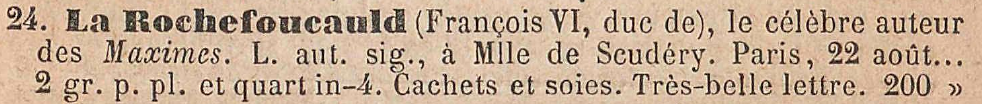
\includegraphics[width=\textwidth]{img/cat_000372_e24.png}
		\caption{Une lettre écrite par La Rochefoucauld vendue à 200 francs.}
		\label{fig:rochefoucauld}
	\end{subfigure}
	\begin{subfigure}{0.8\textwidth}
		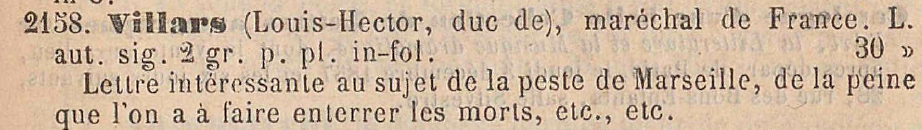
\includegraphics[width=\textwidth]{img/cat_000382_e2158.png}
		\caption{Une lettre écrite par Louis-Hector Villars vendue à 30 francs.}
		\label{fig:villars}
	\end{subfigure}
	\caption{Deux exemples de lettres}
\end{figure}

Pour analyser efficacement la variable \enquote{prix}, il faut pourtant pouvoir, dans une certaine mesure, comprendre les informations implicites et qualitatives contenues dans les catalogues. Le parti pris a donc été de construire le socle de connaissance qui manque à une machine, en s'alignant avec \wkd{} et en s'en servant pour enrichir nos données. Le choix a été fait de ne s'aligner avec \wkd{} que pour certaines parties des entrées de catalogue. Pour rappel, voici leur structure (\ref{code:tei_item}):

\begin{listing}
	\inputminted[linenos, breaklines, tabsize=4]{xml}{code/tei_item.xml}
	\caption{Représentation \xmltei{} d'une entrée de catalogue}
	\label{code:tei_item}
\end{listing}


Les entrées de catalogue contiennent beaucoup d'informations qualitatives, qui pourraient avoir une influence sur le prix du manuscrit: ici par exemple, la description du contenu de la lettre dans le \tnote{}; il est également souvent fait mention du ou de la destinataire. Cependant, l'alignement avec \wkd{} n'a pas été fait avec l'intégralité des entrées. C'est seulement le contenu du \tname{} qui a été aligné avec \wkd{}, à l'aide des informations contenues dans le \ttrait{}. Le \tdesc{} a déjà fait l'objet d'un grand travail de normalisation et d'extraction d'informations; un alignement avec des sources externes n'aurait donc pas une très grande plus-value. L'élément \tnote{} contient souvent des informations intéressantes, puisque c'est là qu'est décrit le contenu d'un manuscrit. Cependant, cet élément n'est pas toujours présent; son contenu est souvent écrit en langage naturel, non structuré, et contient des informations trop variées pour développer un traitement uniforme. Il est donc difficile de tirer parti de cet élément. Le \tname{} et son \ttrait{} sont les éléments les plus régulièrement présents; les informations qu'ils contiennent sont toujours les mêmes (nom d'une personne ou thème d'un manuscrit dans le \tname{}, description du \tname{} dans le \ttrait{}); enfin, ces deux éléments n'ont pas du tout été transformés dans le reste de la chaîne de traitement. Ils portent donc des informations qualitatives centrales pour produire des données exploitables dans une étude économétrique.

Le parti pris a donc été d'aligner avec des identifiants \wkd{} les noms contenus dans les balises \tname{} à l'aide des descriptions contenues dans les \ttrait{}; à partir de cet alignement a été constituée une base de données. Cela permet d'approximer une lecture \enquote{humaine} des items en vente: pour chaque auteur.ice, un certain nombre d'informations auront été récupérées pour mieux identifier la personne (ses occupations, son origine, ses dates de vie...). L'analyse du corpus s'appuit alors sur un bagage de connaissances qui permet d'appréhender par lecture distante l'importance d'une personne. Il devient alors envisageable de voir dans quelle mesure la mention d'une personne impacte le prix d'un manuscrit, et quels sont les facteurs biographiques déterminant dans l'établissement de la valeur. Pour revenir à l'exemple de La Rochefoucauld: à défaut de permettre de savoir qui il est, un alignement avec \wkd{} permet d'identifier son statut et sa place dans la culture française, en récupérant le nombre de ses publications ou encore les institutions dont il est membre.


\subsection{Présentation générale de l'algorithme}
Construire un jeu de données issu de \sparql{} à partir de la manière dont une personne est nommée et décrite au \scl{XIX} n'est pas une opération anodine. La chaîne de traitement est donc assez complexe, comme le montre le schéma \ref{fig:wkdmain}. Cette chaîne de traitement peut être séparée en trois étapes.

\subsubsection{Étape 1 -- Extraction et structuration de données}
Premièrement, il s'agit d'aligner les entrées de catalogue avec des identifiants \wkd{}. Ceux-ci sont liés à des \enquote{entités} \wkd{}: des personnes, lieux et évènements décrits dans \wkd{} par un certain nombre de propriétés (date de naissance, lieu de résidences...). Cette première étape repose avant tout sur l'extraction et la traduction des données depuis les éléments \tname{} et \ttrait{}. Ce processus d'extraction permet de récupérer toutes les données pertinentes pour chaque entrée de catalogue et de les stocker dans un \gls{dictionnaire} structuré. Comme on le verra, la nature \enquote{semi-structurée} des entrées (ainsi qu'une bonne connaissance du corpus) permet de d'automatiser le processus d'extraction et de traduction des données par détection de motifs, sans avoir à passer par l'apprentissage machine: étant donné que les mêmes types d'informations sont toujours présentes et que les entrées suivent des modèles relativement proches, il est possible de s'appuyer sur la structure des entrées pour identifier  les informations pertinentes. L'extraction de données repose donc sur de la détection de motifs à l'aide d'\rgxpl{}: des récurrences sont repérées dans le texte et utilisées pour distinguer différentes informations (nom, prénom, titre de noblesse...). Pour appuyer l'usage d'expressions régulières par une méthode plus \enquote{qualitative} et précise, certains termes particuliers sont extraits et éventuellement traduits à l'aide de \glspl{table de conversion} (c'est-à-dire de \glspl{dictionnaire} qui associent à un terme dans le texte une version normalisée). 

\subsubsection{Étape 2 -- récupération d'identifiants \wkd{} via des recherches en plein texte à l'aide d'une \api{}}
Une fois les données du \tname{} et du \ttrait{} structurées en dictionnaire, elles sont utilisées pour lancer plusieurs recherches en plein texte sur le moteur de recherche de \wkd{}. Ces recherches sont faites automatiquement grâce à l'\api{} de \wkd{}. Pour maximiser les chances d'obtenir un identifiant valide, un algorithme a été conçu pour lancer plusieurs recherches à partir de chaque dictionnaire. La première recherche met bout-à-bout toutes les valeurs disponibles dans le dictionnaire. Ensuite, en fonction des paramètres de recherche disponibles dans le dictionnaire, différentes autres recherches sont lancées. Cet algorithme a été élaboré en menant de nombreux tests pour maximiser le taux de réussite, calculé sous la forme d'un \gls{score F1}.

\subsubsection{Étape 3 -- constitution d'un jeu de données à l'aide de \sparql{}}
Si l'étape d'alignement avec \wkd{} est la plus complexe, elle n'est qu'une étape préparatoire vers la constitution du jeu de données. En fait, récupérer les identifiants est seulement ce qui rend possible l'enrichissement en tant que tel: en lançant une requête \sparql{} sur tous ces identifiants, il est possible, pour chaque entité représentée par l'identifiant, de récupérer des informations depuis \wkd{} et donc de construire le jeu de données définitif. Pour cette étape, le processus est plus simple: les identifiants récupérés à la fin de l'étape précédente sont dédoublonnés (pour éviter de lancer plusieurs fois la même requête); ensuite une requête \sparql{} est initalisée et lancée chacun des identifiants. Les résultats sont traduits depuis les formats \json{} ou \xml{} retournés par \sparql{} sous forme de \json{} plus simple, et donc plus aisément manipulable. Le jeu de données est enregistré dans un fichier. Pour finir, les identifiants \wkd{} sont réinjectés aux catalogues \tei{}, afin de pouvoir faire le lien entre les catalogues et le jeu de données qui a été construit.

Cette chaîne de traitement étant lancée sur plus de 80000 entrées de catalogues, le temps d'exécution est très long et même des petites améliorations de performance peuvent avoir un grand impact; dans sa version initiale, le script demandait des performances particulièrement élevées, et ne fonctionnait pas sur un ordinateur aux capacités limitées. La chaîne de traitement a donc été reprise en plusieurs points afin d'être optimisée, de fonctionner plus vite en étant moins coûteuse en ressources.

\widepage
\begin{figure}[!p]
	\centering
	\tikz[node distance=1cm, scale=0.85, transform shape]{
		\node[db] %
			(db1) at (-5,0)%
			{Source: tableur contenant les \tname{} et \titem{}};
		\node[base]%
			(start) at (0,0)%
			{Lancement de l'algorithme sur toutes les entrées du tableur};
		\draw[arrow] (db1) -- (start);
		
		\node[choice]%
			(detect) at (0,-3.5)%
			{Étape 1 -- extraction de donnée des \tname{} et \ttrait{}};
		\draw[arrow] (start) -- (detect);
		
		\node[transf]%
			(name) at (-4,-6.5)%
			{Extraction et normalisation d'informations nominatives du \tname{}};
		\node[transf]%
			(trait) at (4,-6.5)%
			{Extraction et normalisation d'informations biographiques du \ttrait{}};
		\node[base]%
			(dict) at (0,-9.5)%
			{Constitution d'un dictionnaire structuré pour aligner les \tname{} avec des entités \wkd{}};
		\draw[arrow] (detect) -- (name);
		\draw[arrow] (detect) -- (trait);
		\draw[arrow] (name) -- (dict);
		\draw[arrow] (trait) -- (dict);
		
		\node[db]%
			(logs) at (6,-13)%
			{Optimisation: enregistrement des entrées de catalogues et requêtes déjà traitées};
		\node[transf]%
			(api) at (0,-13)%
			{Étape 2 -- Alogrithme de requêtes sur l'API \wkd{} pour récupérer des identifiants};
		\draw[arrow] (api) -- (logs);
		\draw[arrow] (dict) -- (api);
		
		\node[db]%
			(idset) at (0,-17.5)%
			{Liste d'identifiants \wkd{} à partir de laquelle est constitué le jeu de données};
		\node[transf]
			(sparql) at (0,-20.5)
			{Étape 3 -- Requêtes \sparql{}};
		\node[base]%
			(end) at (0, -23)%
			{Conversion des résultats en \json{} et enregistrement};
		\node[db]%
			(sparqldata) at (5,-23)%
			{Jeu de données issues de \sparql{} au format \json{}};
		\node[transf]%
			(tei) at (0,-25.5)%
			{Réinjection des identifiants \wkd{} dans les fichiers \tei{}};
		\node[db]%
			(teidb) at (-5,-25.5)%
			{Corpus de catalogues en \tei{} augmentés des identifiants \wkd{}};
		\draw[arrow] (api) -- (idset);
		\draw[arrow] (idset) -- (sparql);
		\draw[arrow] (sparql) -- (end);
		\draw[arrow] (end) -- (sparqldata);
		\draw[arrow] (end) -- (tei);
		\draw[arrow] (tei) -- (teidb);
	}
	\caption{\\Présentation générale de l'algorithme d'enrichissement de données à l'aide de \wkd{}}
	\label{fig:wkdmain}
\end{figure}
\restoregeometry

\subsection{Comment traduire des descriptions textuelles datant du XIX\up{ème}~s. en chaînes de caractères qui puissent retourner un résultat sur \wkd{}?} 
Dans la réalisation de cet algorithme, la principale difficulté porte sur la récupération d'identifiants \wkd{} à l'aide de recherches en plein texte. Le script prend en entrée un nom et sa description -- tels qu'elles figurent dans des catalogues datant majoritairement du \scl{XIX}. La difficulté, au delà de la détection et de l'extraction d'informations, est de traduire ces informations pour qu'elles permettent de trouver des résultats pertinents sur \wkd{}. Ce problème est autant linguistique de technique. Une personne ou une chose est nommée ou décrite d'une certaine manière dans un catalogue de vente ancien. Il n'y a aucune garantie que cette caractérisation corresponde à celle faite par \wkd{}: l'orthographe des noms évoluent, tout comme la manière de nommer certains métiers. À ces évolutions orthographiques s'ajoutent des évolutions intellectuelles: les titres de noblesse sont un marqueur plus important au \scl{XIX} français que dans un \scl{XXI} mondialisé. Une personne n'est que rarement décrite par son titre dans \wkd{}. 

\subsubsection{Le problème de la traduction des noms}
Il existe bien sûr des cas simples, comme l'exemple \ref{code:name1}: en extrayant le contenu du \tname et en traduisant le \enquote{roi} issu du \ttrait{}, la chaîne de caractère obtenue est \enquote{Henri IV king}. En recherchant cette chaîne de caractère sur \wkd{}, \href{https://www.wikidata.org/w/index.php?search=Henri+IV+king\&title=Special:Search\&profile=advanced\&fulltext=1\&ns0=1\&ns120=1}{le premier résultat obtenu est correct}. Cependant, de nombreux cas sont plus complexes, surtout lorsque l'auteur.ice du manuscrit est moins célèbre. L'exemple \ref{code:name2} est éclairant: dans le catalogue, la personne est nomée \enquote{Bruno Daru}; sur \wkd{}, le nom de la personne est \enquote{Pierre Daru}, et son nom complet {Pierre Antoine Noël Bruno Daru}. Si la recherche en plein texte est faite avec les mêmes paramètres que pour l'exemple précédent (nom de la personne et titre de noblesse), \href{https://www.wikidata.org/w/index.php?search=bruno+daru+count&title=Special:Search&profile=advanced&fulltext=1&ns0=1&ns120=1}{le premier résultat obtenu} n'est pas le bon: c'est un renvoi à un article de \textit{l'Encyclopedia Britannica} datant de 1911. C'est en cherchant seulement le nom est le prénom que \wkd{} retourne \href{https://www.wikidata.org/w/index.php?search=bruno+daru&title=Special:Search&profile=advanced&fulltext=1&ns0=1&ns120=1}{un résultat pertinent}. Il est intéressant de retenir deux choses de cet exemple: dans les catalogues, le prénom d'une personne correspond en fait souvent à son deuxième ou troisième prénom; ensuite, le titre de noblesse est un critère plus fréquemment mentionné dans les catalogues que dans \wkd{}. Cela s'explique assez aisément: le \scl{XIX} connaît une alternance de régimes politiques (royauté, empire, république) où la noblesse n'a pas encore perdu son pouvoir. La probabilité qu'un titre de noblesse soit mentionné sur \wkd{} diminue lorsqu'un titre est peu important; dans les catalogues, cependant, même les titres les moins importants sont régulièrement mentionnés. Par conséquent, seuls les titres les plus importants seront extraits pour lancer une recherche sur l'\api{} de \wkd{}.

\begin{listing}
	\begin{minted}{xml}
<item n="134" xml:id="CAT_000233_e134">
	<!-- ... -->
	<name type="author">Henri IV</name>
	<trait>
		<p>roi de France.</p>
	</trait>
	<!-- ... -->
</item>
	\end{minted}
	\caption{Un cas simple: Henri IV roi de France}
	\label{code:name1}
\end{listing}

\begin{listing}
	\begin{minted}{xml}
<item n="98" xml:id="CAT_000082_e98">
	<!-- ... -->
	<name type="author">Daru (Bruno, comte)</name>
	<trait>
		<p>célèbre ministre de Napoléon Ier, historien de Venise, de l'Acad. fr., né à Montpellier</p>
	</trait>
	<!-- ... -->
</item>
	\end{minted}
	\caption{Un cas plus complexe: Pierre Antoine Noël Bruno Daru}
	\label{code:name2}
\end{listing}

Dans le cas de noms de personnes étrangères, la situation peut être plus complexe encore. L'exemple \ref{code:name3} combine différentes difficultés.
\begin{itemize}
	\item D'abord, la personne est étrangère; dans les catalogues, les noms sont systématiquement françisés -- \enquote{Albert-Venceslas-Eusèbe} dans le catalogue, \enquote{Albrecht Wenzel Eusebius} en langue originelle. Se pose donc la question de si le nom doit être traduit, et si oui comment? 
	\item Ensuite, comme l'indique la présence de \enquote{dit} dans le \tname{}, il est mentionné un nom de naissance (\enquote{de Waldstein}) et un nom d'usage (\enquote{Wallenstein}). Idéalement, il faudrait choisir entre l'un ou l'autre, plutôt que de rechercher \enquote{Waldstein Wallenstein} sur \wkd{}, ce qui risque d'augmenter le bruit. 
\end{itemize}

Notre approche s'appuyant sur la structure du texte, le deuxième point peut être réglé: le nom d'usage est écrit au début, et le nom de naissance entre parenthèses (c'est également le cas des noms de personnes nobles, par exemple). Il est donc possible de choisir l'un ou l'autre nom. Le premier point est plus problématique: si la traduction du nom serait envisageable en théorie, celle-ci est difficilement compatible avec une approche basée sur la détection de motifs dans le texte: le prénom est repérable comme étant un motif (trois noms séparés par des tirets); cependant, il est impossible de le traduire automatiquement (ce qui demanderait de connaître la langue dans laquelle un prénom doit être traduit). C'est ici que les informations contenues dans le \ttrait{} prennent leur importance: lorsqu'il y a des défaillances dans les informations nominatives, des données biographiques permettent de diminuer le risque d'erreurs. Dans cet exemple, recherche \enquote{Albert-Venceslas-Eusèbe Waldstein} ne \href{https://www.wikidata.org/w/index.php?search=Albert-Venceslas-Eus%C3%A8be+de+Waldstein&title=Special:Search&profile=advanced&fulltext=1&ns0=1&ns120=1}{retourne aucun résultat}, de même que rechercher \href{https://www.wikidata.org/w/index.php?search=Albert-Venceslas-Eus%C3%A8be+Wallenstein&title=Special:Search&profile=advanced&fulltext=1&ns0=1&ns120=1}{Albert-Venceslas-Eusèbe Wallenstein}. Cependant, le bon résultat est obtenu en recherchant \href{https://www.wikidata.org/w/index.php?search=Wallenstein+1634&title=Special:Search&profile=advanced&fulltext=1&ns0=1&ns120=1}{\enquote{Wallenstein 1634}}. Une difficulté supplémentaire vient avec ce type de cas: différents paramètres de recherche (nom, prénom...) ont un impact différent dans l'obtention du bon résultat en fonction des personnes sur qui la requête est faite. Dans ce cas, rechercher le nom d'usage et la date de naissance retourne un résultat valide, ce qui n'est pas toujours le cas. Pour contourner ce problème, trois solutions ont été mises en place: d'abord, ce types de requêtes a été fait \enquote{à la main}, de façon non-automatique, pour de nombreuses entrées différentes afin de déterminer la meilleure combinaison de caractères; ensuite, des tests qui permettent de mesurer l'influence de chaque paramètre de recherche dans l'obtention du résultat; enfin, l'algorithme final lance successivement différentes requêtes avec différents paramètres afin de maximiser la probabilité d'obtenir un résultat valide. Nous reviendrons plus en détail sur les deux derniers points.

\begin{listing}
	\begin{minted}{xml}
<item n="5518" xml:id="CAT_000401_e5518">
	<!-- ... -->
	<name type="author">Wallenstein (Albert-Venceslas-Eusèbe de Waldstein  dit)</name>
	<trait>
		<p>duc de Friedland, célèbre général de la guerre de Trente ans. Assassiné en 1634.</p>
	</trait>
	<!-- ... -->
</item>
	\end{minted}
	\caption{Le problème des noms de personnes étrangères}
	\label{code:name3}
\end{listing}

\subsubsection{L'extraction d'informations biographiques: une autre difficulté}
Cependant, le problème ne s'arrête pas qu'aux noms. Dans un exemple; précédent, le titre de noblesse influençait l'obtention d'un résultat valide. De nombreuses autres informations biographiques pourraient, au premier abord, permettre d'obtenir le bon résultat. C'est souvent le cas, puisque extraire le métier ou la fonction d'une personne permet de supprimer les faux positifs retournés par l'\api{}. C'est par exemple le cas dans l'exemple \ref{code:bio1}. En cherchant uniquement le nom et le prénom (\enquote{Hans Bulow}), le premier résultat retourné renvoie \href{https://www.wikidata.org/w/index.php?search=hans+bulow&title=Special:Search&profile=advanced&fulltext=1&ns0=1&ns120=1}{à un journaliste suédois}. Extraire le mot \enquote{pianiste} \ttrait{} et le traduit en anglais permet d'obtenir \href{https://www.wikidata.org/w/index.php?search=hans+bulow+pianist&title=Special:Search&profile=advanced&fulltext=1&ns0=1&ns120=1}{le bon résultat}.

\begin{listing}
	\begin{minted}{xml}
<item n="136" xml:id="CAT_000189_e136">
	<!-- .. -->
	<name type="author">Bulow (Hans)</name>
	<trait>
		<p>le célèbre pianiste.</p>
	</trait>
</item>
	\end{minted}
	\caption{Un exemple où l'extraction du métier permet l'obtention du bon résultat}
	\label{code:bio1}
\end{listing}

L'extraction d'informations biographiques et leur utilisation dans des requêtes est donc pertinent. Cependant, extraire trop d'informations conduit à lancer des requêtes qui ne renvoient aucun résultat. Dans les exemples \ref{code:bio2} et \ref{code:bio3}, extraire et traduire des fonctions conduit à lancer les requêtes \href{https://www.wikidata.org/w/index.php?search=John+Okey+colonel&title=Special:Search&profile=advanced&fulltext=1&ns0=1&ns120=1}{\enquote{John Okey colonel}} et \href{https://www.wikidata.org/w/index.php?search=Jean+Bouhier+president&title=Special:Search&profile=advanced&fulltext=1&ns0=1&ns120=1}{\enquote{Jean Bouhier president}} qui ne retournent aucun résultat, ou des résultats qui ne sont pas valides. Cependant, dans les deux cas, si une requête est lancée sans la fonction, un résultat correct est obtenu. Les raisons pour lesquelles des résultats erronés sont retournés ne sont cependant pas les mêmes, et il est intéressant de mieux observer les requêtes lancées et les résultats obtenus. Dans le premier cas, le terme mis en avant dans le \ttrait{} (\enquote{colonel}) n'est pas celui avec lequel la personne est décrite sur \wkd{} (où John Okey est décrit comme étant un homme politique). Cela met en avant un problème relatif au changement de regard sur des personnalités: dans un contexte, la personne est décrite comme une figure militaire, dans l'autre comme une figure politique. Le deuxième cas est plus technique. Il y a en fait une erreur dans la requête qui ne retourne pas de résultat (\enquote{Jean Bouhier president}): un.e président.e de parlement n'est en général pas décrite comme \enquote{président}. Cependant, en extrayant des données uniquement par détection de motifs, il est possible de repérer et traduire un terme générique comme \enquote{président}. Extraire le complément \enquote{Parlement de Dijon} du \ttrait{} n'est cependant pas possible (cela impliquerait d'étudier la grammaire de la phrase, pour mettre en avant la relation entre \enquote{président} et \enquote{Parlement de Dijon}). Au vu de la taille et de la variété du jeu de données, il est impossible de traiter au cas par cas des entrées, ou préciser la détection de motif avec suffisamment de précision pour pouvoir résoudre ce genre de difficultés. 

De situations comme les exemples \ref{code:bio2} et \ref{code:bio3}, il faut donc retenir que l'extraction d'informations vient nécessairement avec un risque d'erreur. Le parti pris a donc été de ne pas repérer les métiers et autres termes très spécifiques, comme les grades militaires et les titres de noblesse peu élevés: ils ne retournent pas de résultats sur le moteur de recherche. Ensuite, plus des requêtes sont précises, plus elles risquent de retourner du silence (c'est-à-dire, de ne pas donner de réponse); cependant, si un résultat est obtenu, il est plus probable que ce résultat soit correct. Une fois l'extraction d'informations faite, l'algorithme d'extraction d'identifiants sur l'\api{} \wkd{} a donc été conçu en suivant un principe soustractif: les premières recherches sont faites avec un maximum de paramètres; si aucun résultat n'est obtenu, des paramètres sont enlevés pour que l'\api{} retourne un plus grand nombre de résultats. Enfin, ces deux exemples montrent qu'il n'est pas possible d'extraire et de traduire des informations sans prendre en compte ce qui sera pertinent pour le moteur de recherche de \wkd{}. Il ne s'agit donc pas seulement d'extraire des informations, mais aussi de s'adapter avec ce moteur de recherche pour augmenter la probabilité d'obtenir un résultat valide.

\begin{listing}
	\begin{minted}{xml}
<item n="152" xml:id="CAT_000189_e152">
	<!-- ... -->
	<name type="author">Okey (John)</name>
	<trait>
		<p>colonel anglais, un des lieutenants de Cromwell.</p>
	</trait>
	<!-- ... -->
</item>
	\end{minted}
	\caption{Quand l'extraction d'un métier conduit à des requêtes trop spécifiques}
	\label{code:bio2}
\end{listing}

\begin{listing}
	\begin{minted}{xml}
<item n="5430" xml:id="CAT_000401_e5430">
	<!-- ... -->
	<name type="author">Bouhier (Jean)</name>
	<trait>
		<p>président au Parlement de Dijon, membre de l'Académie française.</p>
	</trait>
	<!-- ... -->
</item>
	\end{minted}
	\caption{Le cas des métiers dont l'extraction est problématique}
	\label{code:bio3}
\end{listing}

% Il faudra donc mettre en place un processus de traduction, depuis le langage naturel en français du \scl{XIX} en anglais adapté aux termes utilisés dans \wkd{}.

\subsection{Comment négocier avec le moteur de recherche de \wkd{}?}
Comme cela commence à apparaître, l'extraction d'informations, lorsqu'elle vise à interagir avec des données externes, vient avec des difficultés supplémentaires. Il ne faut pas seulement extraire les informations ; leur extraction et structuration doivent permettre de lancer des recherches en plein texte, et donc de minimiser le bruit (les informations non pertinentes) et le silence (l'absence d'informations) de la part du moteur de recherche. Il faut donc traduire les informations extraites pour qu'elles correspondent au vocabulaire utilisé par \wkd{}. Cette opération n'est pas anodine: si les catalogues de vente fonctionnent avec leurs propres catégories, le même peut être dit de \wkd{}: certains types de données sont plus souvent référencées que d'autres et \wkd{} utilise un vocabulaire qui lui est propre. Pour bien mener ce processus de traduction et de structuration de l'information, il est nécessaire de bien connaître le fonctionnement de ce moteur de recherche pour mieux s'y adapter.

Comme cela a été dit, l'alignement avec \wkd{} passe par l'utilisation de l'\api{} mise en point par l'institution afin de lancer automatiquement des recherches en plein texte; l'objectif est que le premier résultat retourné par le moteur de recherche soit le bon. La première chose à remarquer est que, contrairement à un moteur de recherche généraliste (comme \textit{Google, QWant}...), ce moteur n'est pas compatible avec des requêtes approximatives. L'exemple \ref{code:search1} est pertinent à ce égard\footnote{Dans cet exemple, le prénom, \enquote{M.-D.-A.}, n'est pas pris en compte pour se concentrer sur l'utilisation d'informations biographiques dans le \ttrait{}.}. Dans de nombreuses entrées, comme c'est le cas ici, les fonctions d'une personne ayant participé à la révolution sont présentées de façon précise: Marc David Alba Lasource est décrit comme étant un \enquote{conventionnel girondin}. Cette mention, régulièrement présente dans les catalogues, pourrait être relevée en tant que telle. Cependant, lancer la recherche \enquote{Lasource conventionnel} ne retourne \href{https://www.wikidata.org/w/index.php?search=lasource+conventionnel&title=Special:Search&profile=advanced&fulltext=1&ns0=1&ns120=1}{aucun résultat}. Si la même recherche est lancée sur un moteur de recherche généraliste (ici, \textit{QWant}), la page \textit{Wikipedia} de Lasource fait partie des premiers \href{https://www.qwant.com/?q=lasource+conventionnel}{résultats}\footnote{Le 29/07/2022, c'est le troisième résultat; le premier correspond à une vente aux enchères d'archives du conventionnel. Les moteurs de recherche pouvant être mis à jour régulièrement, il est possible que l'ordre des résultats change}. Cette différence dans les données retournées par les moteurs de recherche a deux explications: un moteur de recherche généraliste recherche les occurrences de mots, non seulement dans le titre de la page, mais aussi dans le corps du texte. Si le mot \enquote{conventionnel} est absent du titre, il est certainement à plusieurs reprises dans une notice biographique type \textit{Wikipedia}. \wkd{} ne contenant que des données, et pas de texte en tant que tel, l'indexation du corps du texte par le moteur de recherche interne à \wkd{} n'est pas possible. Ensuite, la plupart des moteurs de recherche généralistes utilisent des méthodes de traitement du langage afin de simplifier la requête lancée par l'utilisateur.ice: les mots recherchés sont simplifiés, le moteur de recherche associe les termes recherchés avec d'autres termes \enquote{cooccurents}, c'est-à-dire fréquemment utilisés ensemble\footnote{\cite{noauthor_moteur_2022}. Pour des analyses plus détaillées sur la construction d'ensemble de termes coocurrents via le développement de vecteurs de mots, voir \cite{mikolov_efficient_2013}; pour un article technique détaillant la classification et la sélection de résultats pertinents par apprentissage profond, voir \cite{covington_deep_2016}}. Dans le cas du moteur de recherche de \wkd{}, la requête de l'utilisateur.ice ne semble pas être retraitée: des signes de ponctuation ou des fautes de frappes influencent l'obtention d'un résultat, de même que l'usage de termes inadaptés.

Pour faire face à la \enquote{rigidité} relative du moteur de recherche de \wkd{}, il est donc nécéssaire de préparer ses données au moment de leur extraction. En prenant le même exemple (\ref{code:search1}), un résultat correct peut être obtenu en remplaçant \enquote{conventionnel} par \enquote{politician}\footnote{\enquote{Personnalité politique}}, pour rechercher sur \wkd{} \href{https://www.wikidata.org/w/index.php?search=lasource+politician&search=lasource+politician&title=Special%3ASearch&go=Go&ns0=1&ns120=1}{\enquote{Lasource politician}}. Ici, la traduction de \enquote{conventionnel} en \enquote{politician} est d'autant plus intéressante que la date de naissance dans le catalogue (1762) ne correspond pas à celle indiquée sur \wkd{} (1763). Dans un cas comme celui-ci, où certaines données sont incorrectes, il est important d'extraire un maximum d'informations pour que, si certaines requêtes ne rapportent pas de résultats, pouvoir en faire d'autres avec différents paramètres.

\begin{listing}
	\begin{minted}{xml}
<item n="140" xml:id="CAT_000197_e140">
	<!-- ... -->
	<name type="author">Lasource (M.-D.-A.)</name>
	<trait>
		<p>célèbre conventionnel girondin, né près de Montpellier en 1762, guillotiné en 1793.</p>
	</trait>
	<!-- ... -->
</item>	
	\end{minted}
	\caption{Le problème de l'approximation et de la traduction: Lasource, conventionnel}
	\label{code:search1}
\end{listing}

En conclusion, il faut retenir que le moteur de recherche de \wkd{} n'admet pas d'erreurs, ni de requêtes partiellement erronées (dans l'exemple \ref{code:search1}, où la date de naissance soit correcte, mais pas la date de mort); il ne prend pas non plus en compte la synonymie, ce qui veut dire qu'il n'améliore pas la requête lancée par un.e utilisateur.ice... Cela signifie que les termes utilisés dans une requête doivent être adaptés à ceux que \wkd{} utilise. Les termes spécifiques utilisés dans les catalogues (\enquote{conventionnel}), mais aussi de nombreux titres militaires et de noblesse peu élevés (\enquote{capitaine}, \enquote{marquis}) sont relativement rarement présents sur \wkd{}. Lorsque les requêtes sont lancées, de tels termes sont donc abandonnés et parfois remplacés par des termes plus génériques: par exemple, \enquote{capitaine} est remplacé par \enquote{military}, traduction anglaise de \enquote{militaire}. De même, des termes principalement en usage dans la langue française, comme \enquote{conventionnel} sont moins efficaces pour lancer des recherches.

\subsection{Une approche prédictive}
L'alignement avec \wkd{} et l'extraction d'entités n'est donc pas une opération anodine: les données contenues dans les catalogues sont variées, autant par leur structure que par les informations qu'elles contiennent; il peut être difficile à faire la traduction de données du \scl{XIX} en chaînes de caractères pouvant retourner des réponses valides sur \wkd{}; enfin, le l'alignement repose sur une bonne connaissance du moteur de recherche de \wkd{}. 

De plus, la technique utilisée dans l'extraction de données, reposant sur la détection de motifs à l'aide de \glspl{expression régulière} et de \glspl{table de conversion}, est une technique qui vient avec un certain nombre d'incertitudes. Avec ce genre de techniques, il est impossible de \enquote{comprendre} ce qu'un élément signifie. Dans l'exemple \ref{code:predic}, formellement, rien ne sépare le nom propre de la duchesse (\enquote{Séguier}) du nom de son duché (\enquote{Verneuil}). En s'appuyant sur une connaissance de la structure répétitive des entrées, il est uniquement possible de supposer que le nom entre parenthèses est un nom propre, tandis que le nom hors des parenthèses correspond au nom du duché. En bref, les méthodes de détection de motifs utilisées, peuvent uniquement inférer le sens d'un mot par rapport à sa position dans une phrase. Si cette technique implique une certaine incertitude, elle est cependant particulièrement adaptée à un corpus semi-structuré, comme c'est le cas des catalogues de vente de manuscrits, et à l'opération d'alignement avec \wkd{}. Comme cela est expliqué plus bas, au fond, il n'est pas tellement important de distinguer le sens des différentes informations: ce qui a du sens, c'est que l'extraction et la structuration des informations permet de construire des chaînes de caractères à rechercher sur \wkd{}. Identifier la fonction d'un mot n'est donc ici qu'un moyen -- contrairement à de l'analyse lexicale, où la fonction des mots dans une phrase est signifiante --. En effet, repérer le rôle que tiennent les termes extraits (métier, prénom...) permet de mieux construire la chaîne de caractère recherchée sur \wkd{}, en pouvant filtrer certaines informations (retirer les dates de vie et de mort, par exemple).

\begin{listing}
	\begin{minted}{xml}
<name type="author">Verneuil (Charlotte Séguier duchesse de)</name>
	\end{minted}
	\caption{Peut-on identifier les différents éléments d'une phrase par détection de motifs?}
	\label{code:predic}
\end{listing}

Étant donnée cette quantité d'incertitudes, l'approche suivie dans l'alignement avec \wkd{} peut être qualifiée de \enquote{prédictive}. Par ce terme, il faut comprendre que il n'y a pas, de certitude totale dans le processus d'extraction et de traduction des données. Il n'est pas possible de récupérer avec une certitude totale le bon identifiant. L'objectif cet algorithme n'est donc pas de trouver la \enquote{bonne} réponse. Il est de construire une chaîne de caractère dont on prédit qu'elle apportera un résultat pertinent. De la même manière, la phase de préparation des données est un processus qui sélectionne et normalise certaines informations dont on considère -- après un long processus de test et d'essais -- qu'elles seront pertinentes dans l'obtention des bons résultats. Enfin, le premier rôle des tests est de quantifier les prédictions. Ils répondent à la question: étant donné les résultats obtenus lors des tests, quelle est la probabilité que la prochaine chaîne de caractères recherchée retourne un résultat pertinent? Cette approche prédictive implique nécessairement un degré d'incertitude, et donc le développement d'algorithmes flexibles qui cherchent à minimiser le bruit. 

Être conscient de la nature prédictive de ce processus et quantifier la qualité des algorithmes à l'aide de tests permet cependant de prendre de meilleures décisions techniques. La lecture distante et la détection de motifs supposent d'avancer \enquote{à l'aveugle}, en s'appuyant sur sa connaissance de la structure du texte pour extraire les bonnes informations. Étant donné qu'il est impossible d'être totalement certain que les bonnes données ont été extraites, l'étape suivante -- le lancement des requêtes sur l'\api{} -- doit malléable et s'adapter aux données disponibles. C'est pourquoi le parti pris a été de concevoir un algorithme qui continue de lancer des requêtes en retirant des paramètres tant qu'un identifiant n'a pas été trouvé.

\section{Un algorithme de détection de motifs pour préparer et structurer les données}
\sectionmark{Un algorithme de détection de motifs...}
Avant de chercher à récupérer un identifiant \wkd{} via l'\api{}, un algorithme se charge de traduire et de structurer les données: à partir d'un nom et de son éventuelle description, un dictionnaire qui contient les informations de manière structurée est construit. Cette étape était initialement censée être une simple extraction d'information: à partir du \tname{} et du \ttrait{}, un ensemble d'informations étaient mises bout à bout afin de former une chaîne de caractères à rechercher sur l'\api{}. Le processus s'est complexifié pour intégrer l'extraction, la traduction et la structuration des données. En construisant un \gls{dictionnaire} à partir de texte, il est possible de savoir précisément quelles données sont disponibles pour lancer des requêtes; plusieurs requêtes peuvent alors être lancées sur l'\api{} avec différents paramètres, ce qui permet d'augmenter les probabilités d'obtenir un identifiant valide. 

\subsection{Présentation générale}
\subsubsection{Les formats d'entrée et de sortie}
Le but de l'extraction de données permet de transformer la représentation \tei{}  visible en \ref{code:prepin} -- représentée sous forme d'un \tsv{} pour faciliter la lecture des données -- au \gls{dictionnaire} visible en \ref{code:prepout}. Voici la significtion des différentes clés\footnote{Une clé de \gls{dictionnaire} est l'élément à gauche des \enquote{:}; la clé permet d'accéder à la valeur, visible à droite du \enquote{:}, ce qui permet d'associer des valeurs entre elles, et donc de stocker des objets ou de remplacer une clé présente dans un texte par une valeur, par exemple.} du format de sortie:
\begin{itemize}
	\item \texttt{fname}: cette clé permet d'accéder au prénom d'une personne. Les données contenues dans cette clé viennent du \tname{}. \texttt{fname} est l'abréviation de \enquote{first name}.
	\item \texttt{lanme}: cette clé permet d'accéder au nom de famille de quelqu'un. C'est cette information, extraite du \tname{}, qui est centrale aux requêtes. \texttt{lname} abréviation de \enquote{last name})
	\item \texttt{nobname\_sts}: cette clé contient un nom de famille noble. Dans ces cas, un titre de noblesse est présent dans les entrées de catalogue (seuls les titres de noblesse les plus importants sont extraits du dictionnaire, ce qui n'est pas le cas ici). Les informations contenues ici proviennent du \tname{}. Cette clé est l'abréviation de \enquote{nobility name\_status}
	\item \texttt{status}: le statut d'une personne, soit son titre de noblesse (ici, le titre \enquote{vicomte} n'a pas été extrait car il est rarement présent sur \wkd{}). Les informations contenues ici proviennent en général du \tname{} et parfois du \ttrait{}.
	\item \texttt{dates}: les dates de naissance ou de mort d'une personne (seules ces dates sont conservées). Ces informations proviennent du \ttrait{}.
	\item \texttt{function}: la fonction d'une personne, soit, en général, son métier ou son occupation principale. Cette information provient du \ttrait{}.
	\item \texttt{rebuilt}: un booléen indiquant si un prénom a été reconstruit à partir d'initiales ou non.
\end{itemize}

Comme cela a été dit auparavant, le nom attribué à ces clés n'est pas systématiquement indicateur des valeurs qui y sont associées: si l'entrée de catalogue correspond à une personne, alors les clés correspondent aux informations qu'elles contiennent. Si l'entrée de catalogue ne correspond pas à une personne, ces clés seront également utilisées. Ce qui est important, c'est la hiérarchie d'importance entre les différentes clés: \texttt{lname} est la clé centrale et contient presque toujours des informations, \texttt{fname} des données secondaires et \texttt{date} des dates. Les autres clés sont rarement utilisées si l'entrée de catalogue ne correspond pas à une personne.

\begin{listing}
	\begin{minted}{xml}
<item n="271" xml:id="CAT_000327_e271">
	<!-- ... -->
	<name type="author">Turenne (Henri de La Tour d'Auvergne vicomte de)</name>
	<trait>
		<p>illustre maréchal de France, né en 1611, tué en 1675.</p>
	</trait>
	<!-- ... -->
</item>
	\end{minted}
	\caption{L'entrée \xmltei{} à partir de laquelle des données sont extraites}
	\label{code:prepin}
\end{listing}

\begin{listing}
	\begin{minted}{python}
{
	"fname": "henri ", 
	"lname": "la tour d'auvergne", 
	"nobname_sts": "Turenne ", 
	"status": "", 
	"dates": "1611 1675 ", 
	"function": "marshal", 
	"rebuilt": False
}
	\end{minted}
	\caption{La sortie \json{} correspondante}
	\label{code:prepout}
\end{listing}

\subsubsection{Présentation de l'algorithme d'extraction d'informations}
L'algorithme détaillé ci dessous est présenté sous forme graphique dans la figure \ref{fig:extractmain}. Cette étape peut être séparée en deux parties différentes: l'extraction d'informations nominatives du \tname{} et la récupération de données biographiques du \ttrait{}.

L'extraction d'informations du \tname{} est l'étape plus complexe. La difficulté tient au fait que cette balise peut contenir des informations variées et structurées de façon très différente. Cela demande d'identifier des motifs récurrents et de les repérer dans le texte à différents degrés et à différentes étapes. Dans un premier temps, les prénoms sont systématiquement extraits. Ils sont toujours détectés -- même si la balise ne contient le nom d'une personne: cette extraction permet justement d'identifier le type de données contenues dans le \tname{}. Les prénoms sont repérés à l'aide de plusieurs \glspl{expression régulière} qui permettent d'identifier des prénoms complets et abrégés, qu'ils soient composés ou non. Cette détection prend en compte les différents types d'abréviations possibles (un prénom composé peut être entièrement abrégé; à l'inverse, seulement un des prénoms peut être abrégé) et les différentes typographies (séparer les prénoms avec des traits d'union ou non, par exemple). Dans le cas où un prénom serait abrégé, il est si possible reconstruit: des initiales sont remplacées par un nom complet; ce processus est présenté plus en détail ci-dessous. Cela permet d'augmenter le taux de réussite dans l'alignement avec des identifiants \wkd{}, mais vient avec plusieurs difficultés techniques, comme nous le verrons. Une fois ce nom extrait, le type d'information contenue dans le \tname{} doit être identifié: en fonction du type d'information (géographique, historique, nominative...), différents traitements sont mis en place. Cette identification se fait par détection de motifs augmentée par l'usage de \glspl{table de conversion}\footnote{Pour un exemple de table de conversion, voir \ref{appendix:convfunction}} et de listes contenant du vocabulaire spécifique. Listes et tables étant classées thématiquement, il est possible, par un processus éliminatoire, d'identifier avec certitude le type d'information contenue dans le \tname{}. Le traitement du \tname{} dépend grandement de cette détection: si cette balise contient des éléments géographiques ou historiques, l'extraction d'informations repose en grande partie sur les tables de conversion. S'il s'agit en revanche d'un nom de personne, il est alors nécessaire d'identifier les différents types de données nominatives (prénom, nom de famille, nom de famille noble...) pour bien structurer les données. En effet, c'est de cette structure que dépend la bonne construction du \gls{dictionnaire}, et donc la constitution de requêtes adaptées à l'\api{}. Ce processus d'extraction des données s'appuie majoritairement sur une détection de motifs. Le motif déterminant est la présence ou non dans parenthèses dans le nom. Comme nous le verrons, si un nom contient des parenthèses, les informations sont bien plus structurées que s'il n'en contient pas. Les informations peuvent alors être extraites avec une bien plus grande granularité.

Une fois les informations nominatives extraites du \tname{}, il reste à extraire les données biographiques pertinentes du \ttrait{}. Cette étape, plus simple que la précédente, vaut principalement pour les entrées où c'est l'auteur.ice d'un document qui est mentionné.e dans le \tname{}. Les seules informations extraites concernent les dates de vie et de mort des personnes, ainsi que son métier. Quelques difficultés techniques subsistent cependant: il faut notamment distinguer une date de naissance/décès d'une autre date, afin de diminuer le bruit; de plus, il faut réussir à extraire de façon automatique l'occupation principale d'une personne, lorsque plusieurs personnes sont mentionnées (\enquote{militaire} et \enquote{auteur}, par exemple). La résolution de ces deux problèmes repose sur une bonne connaissance du corpus de catalogues et de la structure des \ttrait{}.



\widepage
\begin{figure}[!p]
	\centering
	\tikz[node distance=1cm, scale=0.70, transform shape]{
		\node[db]%
			(input) at (-12,2)%
			{Données en entrée};
		\node[base]%
			(start) at (-3,2)% 
			{Lecture des données et lancement de l'algorithme};
		\node[base]%
			(tname) at (-3,0)%
			{Étape 1 -- Extraction de données du \tname{}};
		\node[transf]%
			(rebuild) at (7,-4)%
			{Extraction du prénom et reconstruction d'un prénom complet à partir de sa version abrégée};
		\node[choice]%
			(type) at (-3,-4)%
			{Détection du type de \tname{}};
		\draw[arrow] (input) -- (start);
		\draw[arrow] (start) -- (tname);
		\draw[arrow] (tname) -- (type);
		\draw[arrow] (tname) -- (7,0) -- (rebuild);
		
		\node[base]%
			(meme) at (-12, -8)%
			{Même personne que l'entrée précédente};
		\node[transf]%
			(memetr) at (-12, -11)%
			{Réutilisation du dictionnaire de l'entrée précédente; le script passe à l'entrée suivante};
		\draw[arrow] (type) -- (meme);
		\draw[arrow] (meme) -- (memetr);
		
		\node[base]%
			(div) at (-7,-8)%
			{Pas d'informations (ex: \enquote{Divers})};
		\node[transf]
			(divtr) at (-7,-11)%
			{Pas d'extraction d'informations};
		\draw[arrow] (type) -- (div);
		\draw[arrow] (div) -- (divtr);
		
		\node[base]%
			(pers) at (-2,-8)%
			{\tname{} contenant le nom d'une personne};
		\node[choice]%
			(persch) at (-2,-14)%
			{Détection du type de nom: avec/sans parenthèses};
		\node[transf]%
			(nopartr) at (-5, -19)%
			{Nom sans parenthèses: nettoyage simple des données \\ Réinjection du prénom extrait au début dans le \texttt{fname} et du reste dans le \texttt{lname}};	
		\node[transf]%
			(partr) at (1, -19)%
			{Nom avec parenthèses: voir \ref{fig:extractparenthesis} \\ Injection du prénom extrait en entrée du script};
		\draw[arrow] (type) -- (pers);
		\draw[arrow] (pers) -- (persch);
		\draw[arrow] (persch) -- (nopartr);
		\draw[arrow] (persch) -- (partr);
		
		\node[base]%
			(geo) at (3,-8)%
			{\tname{} avec informations géographiques};
		\node[transf]%
			(geotr) at (3,-11)%
			{Extraction d'informations à l'aide de tables de correspondance et ajout au \texttt{lname}};
		\draw[arrow] (type) -- (geo);
		\draw[arrow] (geo) -- (geotr);
				
		\node[base]%
			(hist) at (8,-8)%
			{\tname{} historique};
		\node[transf]%
			(histtr) at (8,-11)%
			{Extraction d'informations à l'aide de tables de correspondance et ajout au \texttt{lname}};
		\draw[arrow] (type) -- (hist);
		\draw[arrow] (hist) -- (histtr);
		
		\node[base]%
			(ttrait) at (-2,-23)%
			{Étape 2 -- Extraction de données du \ttrait{}};
		\node[transf]%
			(date) at (-5,-25)%
			{Extraction des dates de vie et de mort et ajout au \texttt{date}};
		\node[transf]%
			(func) at (1,-25)%
			{Extraction et traduction du métier et ajout au \texttt{function}};
		
		\node[base]%
			(end) at (-2,-27)%
			{Dictionnaire structuré pour lancer les requêtes};
		
		\begin{pgfonlayer}{bg} % \draw on the background of nodes
			\draw[dotted] (rebuild) -- (7,-6.5) -- (0.75,-6.5) -- (partr);
			\draw[dotted] (rebuild) -- (7,-6.5) -- (-4.5,-6.5) -- (nopartr);
			\draw[arrow] (divtr) -- (-7,-23) -- (ttrait);
			\draw[arrow] (nopartr) -- (-5,-23) -- (ttrait);
			\draw[arrow] (partr) -- (1,-23) -- (ttrait);
			\draw[arrow] (geotr) -- (3,-23) -- (ttrait);
			\draw[arrow] (histtr) -- (8,-23) -- (ttrait);
			\draw[arrow] (ttrait) -- (date);
			\draw[arrow] (ttrait) -- (func);
			\draw[arrow] (date) -- (-5,-27) -- (end);
			\draw[arrow] (func) -- (1,-27) -- (end);
			\draw[arrow] (memetr) -- (-12,-27) -- (end);
		\end{pgfonlayer}
	}
	\caption{Processus d'extraction d'informations du \tname{} et \titem{}}
	\label{fig:extractmain}
\end{figure}
\restoregeometry

\widepage
\begin{figure}[!p]
	\centering
	\tikz[node distance=1cm]{
		\node[base](start) at (0,0)%
			{\tname{} contenant des parenthèses};
		\node[base] (fname) at (8,0)%
			{Prénoms extraits du \tname{} et éventuellement reconstruits};
		\node[label={[rotate=-90]below:Réinjection des prénoms déjà extraits}] at (8.75,-4.25) {};
			
		\node[choice](nobl) at (0,-3)%
			{Est-ce que le \tname{} contient un titre de noblesse?};
		\node[label={OUI}] at (-2.25,-5.25) {};
		\node[label={NON}] at (2.25, -5.25) {};
 		
		\node[transf](y1) at (-4,-8)%
			{Extraction des données entre parenthèses: titre de noblesse (ajouté au \texttt{status}) et nom de famille personnel ajouté au \texttt{lname}};
		\node[transf](y2) at (-4,-13)%
			{Injection des prénoms extraits à l'épape précédente dans le \texttt{fname}};
		\node[transf](y3) at (-4,-17.5)%
			{Extraction des données en dehors des parenthèses: le nom de famille noble, ajouté au \texttt{nobname\_sts}};
		
		\node[transf](n1) at (4,-8.5)%
			{Extraction des données entre parenthèses: seconde extraction de prénoms pour réduire le bruit et nettoyage};
		\node[transf](n2) at (4,-13.5)%
			{Réinjection des prénoms extraits et combinaison des prénoms extraits pour constituer le \texttt{fname}};
		\node[transf](n3) at (4,-17.5)%
			{Extraction du nom de famille hors parenthèses et constitution du \texttt{lname}};
			
		\node[base](end) at (0,-21)%
			{Passage à l'extraction d'informations du \texttt{lname}};
		
		\begin{pgfonlayer}{bg} % \draw on the background of nodes
			\draw[arrow] (start) -- (nobl);
			\draw[arrow] (nobl) -- (y1);
			\draw[arrow] (y1) -- (y2);
			\draw[arrow] (y2) -- (y3);
			\draw[arrow] (nobl) -- (n1);
			\draw[arrow] (n1) -- (n2);
			\draw[arrow] (n2) -- (n3);
			\draw[arrow] (n3) -- (4,-21) -- (end);
			\draw[arrow] (y3) -- (-4,-21) -- (end);
			\draw[dotted,] (fname) -- (8,-13.5) -- (n2);
			\draw[dotted] (fname) -- (8,-11) -- (-3.5,-11) -- (y2);
		\end{pgfonlayer}	
	}
	\caption{Extraction d'informations d'un \tname{} contenant des parenthèses}
	\label{fig:extractparenthesis}
\end{figure}
\restoregeometry

\subsection{Identifier le type de nom}
Les éléments \texttt{tei:name} contiennent le titre donné à l'item vendu. Si c'est souvent le nom de l'auteur.ice du document, ce n'est pas toujours le cas. L'extraction d'éléments du \tname{} dépend, comme cela a été dit, de l'identification du \enquote{type} de nom. La décision a été prise de classer tous les \tname{} en cinq catégories.

Les noms génériques: ces éléments ne contiennent pas d'informations précises. Les entités \wkd{} étant spécifiques plutôt que génériques, il n'est pas certain que les entrées puissent être alignées avec \wkd{}; si des entités \wkd{} correspondent  à ces éléments, les informations qu'elles contiennent seront probablement trop génériques pour être utilisables dans un contexte économétrique. Lorsque cela est possible, l'alignement est quand même fait; c'est le cas par exemple pour les \tname{} contenant la mention de chartes. Dans ces cas, un dictionnaire vide est retourné et l'alignement avec \wkd{} n'aura pas lieu. Une exception est faite dans le cas chartes, où un alignement est fait avec l'entité \wkd{} génériques. Dans cette catégorie se trouve par exemple: 
\begin{itemize}
	\item \mintinline{xml}|<name type="author">DIVERS</name>|
\end{itemize}

Les noms de type \enquote{Le même} ou \enquote{La même}; lorsqu'il y a cette valeur dans le \tname{}, l'auteur.ice est la même personne que l'auteur.ice de l'entrée de catalogue précédente. Dans ce cas, le dictionnaire de cette entrée est réutilisé. Par exemple:
\begin{enumerate}
	\item \mintinline{xml}|<name type="author">Le même</name>|.
\end{enumerate}

Les noms géographiques; ces entrées sont détectées à l'aide de tables de conversion et de listes. Celles-ci sont classées thématiquement: liste d'anciennes colonies françaises (\ref{appendix:convcolonie}), de départements français du \scl{XIX}(\ref{appendix:convdpt}), d'anciennes provinces françaises (\ref{appendix:convprov}) et de pays (\ref{appendix:convcountry}). Dans ce cas, un alignement avec une entité \wkd{} est possible; cependant, il n'est pas toujours envisageable de retrouver l'entité précise. En effet, un \tname{} peut contenir une mention d'une donnée géographique, mais également d'autres détails. C'est par exemple le cas dans le quatrième exemple ci-dessous. Il faut alors aligner le \tname{} avec son équivalent générique sur \wkd{} (l'exemple ci-dessous, par exemple, a été aligné uniquement avec l'entité \enquote{Paris}). Dans cette catégorie se trouvent:
\begin{itemize}
	\item \mintinline{xml}|<name type="other">AISNE (département de 1')</name>|
	\item \mintinline{xml}|<name type="author">Bourbonnais. </name>|
	\item \mintinline{xml}|<name type="author">Paris : Musée royal du Louvre</name>|
	\item \mintinline{xml}|<name type="author">Garde nationale parisienne en 1792 (brevet|
\end{itemize}
\begin{itemize}[label={}]
	\item \mintinline{xml}|de volontaire de la)</name>|
\end{itemize}

Les noms correspondant à des évènements historiques. Là encore, une table de conversion est utilisée (\ref{appendix:convevt}). Ici, une difficulté apparaît cependant: du fait de la varité des évènements historiques mentionnés dans les entrées de catalogue, il n'est pas possible d'enregistrer l'ensemble des évènements dans des tables afin de permettre une détection de tous les évènements. Les \tname{} ont donc été analysés pour extraire les évènements les plus importants. Ensuite, comme pour les termes géographiques, il n'est pas possible de donner aux tables de conversion une granularité suffisamment fine pour contenir toutes les données possibles. Des alignements partiels ont donc été faits: le premier exemple ci-dessous a été aligné avec l'entité \wkd{} \enquote{Révolution française}.
\begin{itemize}
	\item \mintinline{xml}|<name xmlns="http://www.tei-c.org/ns/1.0" type="other">THÉATRE|
\end{itemize}
\begin{itemize}[label={}]
	\item \mintinline{xml}|RÉVOLUTIONNAIRE</name>|
\end{itemize}
\begin{itemize}
	\item \mintinline{xml}|<name type="author">COMMUNE DE 1871.</name>|
	\item \mintinline{xml}|<name type="other">Siège de La Rochelle en 1628</name>|
\end{itemize}

Les noms de personnes. Ceux-ci ne sont pas simples à traiter: ils peuvent contenir de nombreuses informations: deux noms de famille (usuels et nobles), titres de noblesse, plusieurs prénoms. Ils ont également une structure variée, comme cela apparaît dans les exemples ci-dessous: les noms peuvent être écrits en utilisant des parenthèses ou non; un prénom peut être écrit en entier, comme dans premier exemple, entièrement abrégé (comme dans l'exemple 3) ou encore partiellement abrégé, ce qui est le cas dans le troisième exemple. Ces différences, qui ne posent pas de problème à un regard humain, sont autant de problèmes techniques. En effet, la détection de motifs fonctionne uniquement sur des critères formels, ou structurels. Il faut donc, en s'appuyant sur la structure des documents, réussir à distinguer un prénom d'un nom de famille, un nom de famille d'un autre, ou encore un nom abrégé d'un nom complet.
\begin{itemize}
	\item \mintinline{xml}|<name type="author">Humboldt (le baron Alexandre de)</name>|
	\item \mintinline{xml}|<name type="author">Taccani Tasca (madame la comtesse)</name>|
	\item \mintinline{xml}|<name type="author">LEGOUVÉ (G. M. J. B.)</name>|
	\item \mintinline{xml}|<name type="author">LOUIS XVIII</name>|
	\item \mintinline{xml}|<name type="author">Duras (Emm.-F. de Durfort, duc de)</name>|
\end{itemize}

Si l'on pose l'extraction d'informations nominatives sur une personne comme étant l'objectif principal, une difficulté apparaît vite: qu'est-ce qui distingue un nom de personne d'un des autres types de noms? Les éléments \tname{} sont voués à contenir des noms propres; chercher à distinguer les noms propres des noms communs n'a donc pas d'intérêt. Cela est d'autant plus que la graphie varie d'un catalogue à l'autre: dans certains, les majuscules sont signifiantes et pourraient permettre de distinguer noms communs et noms propres, tandis que dans d'autres, l'intégralité du \tname{} est en majuscule. Une détection de motifs à partir de simples critères formels (du type: \enquote{Un nom de personne est un ou plusieurs mots commençant par des majuscules}) n'est pas opérante pour ce corpus. Il n'est pas non plus possible de définir un nom positivement, puisqu'il n'existe aucun critère définitoire pour un nom propre. Enfin, à cette étape, il n'est pas non plus possible de s'appuyer sur l'extraction de prénoms. L'extraction de prénoms se base, comme on le verra, sur de la détection de motifs; là encore, ce qui est identifié comme un prénom peut tout aussi bien être un nom propre, et il n'existe à ce stade aucune possibilité pour distinguer un nom propre d'un autre. C'est à ce stade qu'a été décidée l'utilisation de tables de conversion et de listes contenant du vocabulaire thématique: en identifiants des références récurrentes à des évènements ou des lieux dans les \tname{}, il devient possible de définir les noms de personne négativement. En définitive, un nom de personne, c'est donc ce qui n'est pas autre chose et la détection du type de nom fonctionne donc de manière éliminatoire.

L'algorithme mène donc une série de tests, cherchant à détecter si un \tname{} rentre dans telle ou telle catégorie. Du fait du fonctionnement technique de \py{}, une série de tests éliminatoires doit aller du cas le plus particulier au cas le plus générique afin d'éviter les faux positifs: une fois qu'un élément a été détecté comme appartenant à une catégorie, il ne peut plus être réassigné à une autre. C'est pourquoi l'algorithme commence par chercher à classer les éléments dans les catégories où le taux d'erreur est le plus faible, pour ensuite finir par la catégorie la plus générique: celle des noms de personne.: c'est dans ces catégories que le taux d'erreur est le plus faible. 

Le script commence donc par chercher à classer un \tname{} dans les catégories où les informations sont écrites plus ou moins toujours de la même manière. Il cherche d'abord à identifier si le \tname{} correspond à \enquote{Le même} ou \enquote{La même}. Dans ce cas, le \tname{} est le même que celui de l'entrée précédente et c'est ce \gls{dictionnaire} qui est réutilisé. Ensuite, les entrées génériques sont détectées. Comme elles contiennent toujours des informations écrites de la même manière (\enquote{Documents divers}), le taux d'erreur est là encore très faible. Ces entrées génériques ne contiennent pas d'informations spécifiques; si un \tname{} appartient à cette catégorie, alors l'algorithme n'extrait pas d'informations. 

Ensuite, si un \tname{} n'appartient ni à l'une ni à l'autre catégorie, alors l'algorithme cherche à classifier un nom en différentes catégories à l'aide de tables de comparaison et de listes contenant du vocabulaire spécifiques. Ces tables et listes sont classées en deux catégories (données historiques et géographiques) afin de définir des traitements spécifiques; l'algorithme cherche d'abord à identifier des entrées géographiques, puis historiques. En effet, un bien plus grand nombre de tables contenant des données géographiques existe\footnote{Nom d'anciennes provinces françaises (\ref{appendix:convprov}), de départements du \scl{XIX} (\ref{appendix:convdpt}), d'anciennes colonies (\ref{appendix:convcolonie}) et de pays (\ref{appendix:convcountry})}, ce qui augmente les possibilités d'un classement correct. Enfin, le script cherche à identifier des informations historiques dans un \tname{} (\ref{appendix:convevt}). Si une donnée géographique ou historique est repérée, alors équivalents normalisés de cette donnée sont ajoutés au \gls{dictionnaire} grâce à l'usage de tables de conversions. 

Par processus d'élimination, si aucune de ces informations n'a été détectée, alors il n'est plus possible de classer le \tname{} dans aucune autre catégorie. Il est alors considéré que le contenu du \tname{} est le nom d'une personne. L'extraction d'informations se fait ici plus complexe \footnote{Pour une représentation graphique de cette étape, voir \ref{fig:extractparenthesis}}, comme nous le verrons: le script traite le nom différemment en fonction de sa structure (présence ou non de parenthèses dans le nom), puis extrait d'éventuels titres de noblesse, noms de famille noble et nom de famille usuel. Enfin, il extrait des prénoms et cherche à reconstruire un prénom complet à partir de son abréviation. Le processus étant éliminatoire, il n'y a bien sûr aucune certitude totale que le contenu du \tname{} soit bel et bien le nom d'une personne; il n'est cependant plus possible de mieux catégoriser les éléments. Cela n'est pas non plus extrêmement important, puisque cet algorithme de classification a un rôle fonctionnel et n'impacte pas la manière dont les identifiants sont récupérés depuis l'\api{} \wkd{}. Il permet principalement d'adopter un fonctionnement modulaire en cherchant à détecter des motifs spécifiques dans les \tname{} en fonction de la catégorie à laquelle ils appartiennent. La détection de motifs étant \enquote{aveugle}, le traitement qui est fait pour cette catégorie peut être mis à profit de différents types de données: les mêmes motifs peuvent être recherchés et extraits de différents types d'entrées.

À l'issue de cette phase de classification, il est possible de mieux connaître les types de \tname{} et leur répartition dans le corpus. Les noms de personnes sont très majoritaires dans les \tname{}: ils représentent 73305 entrées sur un total de 82913, soit 81,52\%. C'est pour ce type de données que l'extraction des données a été pensée; les informations sont donc extraites avec une granularité plus fine qu'avec le reste du corpus. Viennent ensuite les noms de lieux (8693 entrées) et les éléments divers (550). Pour finir se trouvent les évènements historiques (232 entrées) et les éléments vides\footnote{Ces chiffres proviennent d'un calcul réalisé à partir du script développé pour identifier le type d'entrée. Ils ont été produits afin de réaliser une représentation graphique du type d'entrée, visible en annexes (\ref{appendix:tnametypes})}.


\subsection{Le traitement des noms de personnes}
Peut-être y intégrer la subsection suivante ?
\ref{fig:extractparenthesis} (qui contient une sous-partie de l'algorithme pour plus de lisibilité)


\subsection{Reconstruire un prénom complet à partir de son abréviation}
Souvent, le prénom d'une personne est écrit en abrégé. Partant de ce constat, un algorithme a été construit pour:
\begin{itemize}
	\item Repérer lorsqu'un prénom est abrégé, en prenant en compte différents types d'abréviations (nom simple ou composé, nom entièrement ou partiellement abrégé) et des possibles fautes dans les catalogues (un point est oublié à la fin d'une abréviation, par exemple).
	\item Reconstruire un prénom complet à partir de son abréviation, ce qui passe pas un algorithme qui cherche à reconstruire le nom en plusieurs étapes pour obtenir le nom le plus complet possible avec un mimimum d'erreurs.
\end{itemize}

Ici, l'approche est totalement prédictive: il est impossible d'être certain d'obtenir le bon nom complet à partir de son abréviation; on peut uniquement prédire que le prénom reconstruit sera conforme au vrai prénom (tel qu'il est écrit sur \wkd{}) et chercher à maximiser cette certitude.

\subsection{Extraire des informations normalisées à partir d'un nom et de sa description}
Cette sous-section détaille l'utilisation de tables de conversion pour traduire et normaliser certaines donnes importantes (dates de vie et mort, titres de noblesse et fonctions).

BIEN PENSER à parler du problème des informations extraites, mais qui ne se rattachent pas à la personne du \tname{} (eg: femme du comte...) => comment, par détection de motifs, est-ce que l'on règle le problème.

\section{Extraire des identifiants \wkd{}}
Une fois un dictionnaire de données normalisées produites, un algorithme lance des recherches en plein texte sur l'\api{} de \wkd{} afin de récupérer des identifiants. L'algorithme lance plusieurs requêtes successivement. L'objectif est de récupérer un identifiant en lançant le moins de requêtes, avec le plus de certitude possible.

\subsection{Présentation générale}
Ici est présenté le fonctionnement général de l'algorithme, qui se comporte différemment en fonction du type de données qu'il a à traiter (personne noble ou non, prénom reconstruit ou non...).

\subsection{Gérer la montée en charge: optimisation et réduction du temps d'exécution}
Le script est assez compliqué, repose sur une \api{} et traite un grand nombre de données (plus de 82000 entrées). Il prend donc plus d'une dizaine d'heures à s'exécuter et demande des ressources élevées (la première version du script ne fonctionnait plus sur mon ordinateur après avoir traité 5\% du jeu de données). L'optimisation nécessaire de l'algorithme est décrite dans cette sous-section.

\subsection{Évaluation du script : tests, performance et qualité des données extraites de \wkd{}}
Des tests ont été réalisés pour:
\begin{itemize}
	\item isoler l'impact de chaque paramètre (élément du dictionnaire) dans l'obtention des bons résultats
	\item évaluer la qualité de l'algorithme final
	\item mesurer la performance de celui-ci.
\end{itemize}
Ces tests, et leurs résultats, sont présentés ici.

\section{Après l'alignement, l'enrichissement: utiliser \sparql{} pour produire des données structurées}
La récupération des identifiants \wkd{} est la partie la plus complexe dans l'utilisation de \wkd{} pour enrichir des données. Après une présentation des informations requêtées via \sparql{}, le processus d'extraction d'informations et de stockage dans un \json{} est détaillé.

\subsection{Quelles données rechercher via \sparql?}
Après avoir expliqué pourquoi développer des méthodes d'enrichissement automatique, une seconde question se pose: quelles sont les données à récupérer? Cette question n'est pas anodine du fait de la diversité du corpus. Le titre donné à un manuscrit dans un catalogue et inscrit dans le \tname{} est souvent celui d'une personne, mais ce n'est pas toujours le cas. Il arrive également qu'un manuscrit soit nommé d'après un évènement (la Révolution française), un lieu ou une province (Italie, Poitou), ou encore une typologie de document (des chartes).

Un bref retour sur la manière dont fonctionne \sparql{} permet de mieux comprendre le problème que peut poser la diversité du corpus. \sparql{} a l'avantage de permettre de récupérer des données propres sur des bases de données en ligne; cependant, l'information y est organisée de manière très spécifique, ce qui demande de faire des requêtes précises. Ce langage de requêtes a pour but d'interagir avec une base de données au format \rdf{}. Avec ce format -- dit sémantique -- les données sont organisées en \enquote{triplets} sujet--prédicat--objet, où:

\begin{itemize}
	\item le sujet est la ressource principale.
	\item le prédicat est une propriété du sujet, qui caractérise une relation avec une autre ressource, l'objet.
	\item l'objet est une ressource secondaire: c'est la valeur d'un prédicat.
\end{itemize}

Le principe des triplets \rdf{} est mieux exprimé sous forme graphique (\ref{fig:triplet}):

\begin{figure}[!h]
	\centering
	\tikz{
		\node%
		[base] %
		(S) at (0,0) %
		{\textbf{Sujet} \small \\ La ressource principale \\ \textit{Natalia Gontcharova}};
		\node%
		[transf] %
		(P) at (5, 0) %
		{\textbf{Prédicat} \small \\ La relation à l'objet \\ \textit{a peint}};
		\node%
		[base] %
		(O) at (10, 0) %
		{\textbf{Objet} \small \\ Une ressource secondaire \\ \enquote{\textit{Les porteuses}}};
		
		\draw[arrow] (S) -- (P);
		\draw[arrow] (P) -- (O);
	}
	\caption{Exemple de relation sujet -- prédicat -- object}
	\label{fig:triplet}
\end{figure}

Deux particularités supplémentaires définissent les formats sémantiques:
\begin{itemize}
	\item Toutes les \enquote{ressources} peuvent être tour à tour sujet ou objet. L'exemple du dessus, par exemple, aurait pu être réécrit sous la forme: \enquote{Les porteuses} a été peint par Natalia Gontcharova. Dans ce cas, Natalia Gontcharova est l'objet et \textit{Les porteuses} est le sujet. Par conséquent, une base de données \rdf{} est une base de donnée en graphes; elle peut être représentée sous la forme d'un réseau de ressources qui entretiennent des relations bilatérales entre elles. Il n'y a pas de hiérarchie entre les informations, contrairement à une base de données \xml{} classique.
	\item L'ensemble des ressources et des prédicats d'une base de donnée en graphe sont définis et disposent d'un identifiant unique. Les prédicats, plus particulièrement, sont définis selon une ontologie particulière.
\end{itemize}

Le deuxième point complexifie la définition des données à récupérer via \sparql{}: les prédicats sont décrits avec une grande précision; par conséquent, une information analogue peut être représentée par différents prédicats dans différentes situations. Dans l'ontologie \wkd{}, la création d'un texte et la création d'une peinture ne correspondent pas au même prédicat. Pour que les données soient utilisables, il faut être très spécifique quant aux informations recherchées. 

Les 18899 entités avec lesquelles les entrées de manuscrits ont été alignées peuvent se classer en de nombreuses catégories. Sur \wkd{}, une entité est une \enquote{instance} d'une classe plus large. En suivant la classification de \wkd{}, les entités appartiennent aux catégories suivantes\footnote{Un graphique présentant l'ensemble de ces catégories se trouve en annexes (\ref{appendix:wikidata_instances}).}:
\begin{itemize}
	\item personnes humaines; cette catégorie est la plus fréquente (12090 occurrences)
	\item noms de familles (3180 entités)
	\item communes françaises (586 occurrences)
	\item peintures et sculptures (respectivement 520 et 236 entités)
\end{itemize}

Cette variété peut s'expliquer en partie par le taux d'erreur dans l'alignement avec Wikidata. Cependant, toutes ces \enquote{erreurs} ne correspondent pas forcément à des résultats qui ne sont pas pertinents. Par exemple, l'algorithme peut aligner un.e écrivain.e avec un de ses ouvrages, ou une personne avec son portrait. Des résultats erronés peuvent toujours garder une forme de pertinence. Il est d'autant plus important de construire des requêtes \sparql{} qui se concentrent pas uniquement sur des personnes. Cependant, il n'est pas possible de faire une requête qui correspondent à toutes les catégories auxquelles appartiennent le corpus. Le choix a donc été fait de se concentrer sur les catégories les plus pertinentes: les personnes, les familles, et les œuvres artistiques et littéraires. Non seulement ces catégories contiennent la grande majorité du corpus (16026 entités), mais ces catégories sont les plus à même de contenir des entités pertinentes. Il a été choisi de ne pas faire de requête spécifique sur les lieux, puisque peu d'informations sont disponibles pour les entités de la catégorie \enquote{communes françaises} sur Wikidata.

Un nombre assez conséquent de données ont donc été requêtées avec \sparql{}, du fait des spécificités des bases de données en graphes, de la variété des entités \wkd{} auxquelles les manuscrits sont liées, et enfin du fait de la variété du corpus lui même. Ces informations récupérées correspondent aux différentes catégories de \wkd{}.
\begin{itemize}
	\item Pour les personnes et les familles, les informations suivantes sont récupérées sur \wkd{}:
	\begin{itemize}
		\item Le genre de la personne;
		\item Sa nationalité, afin de voir si l'origine d'une personne influence le prix d'un manuscrit;
		\item Les langues parlées par une personne; là encore, l'objectif est d'étudier l'impact de l'origine d'un.e auteur.ice sur un prix.
		\item Les date de vie et de mort, afin de placer un manuscrit dans une époque et de voir comment son ancienneté et sa contemporanéité en influencent le prix.
		\item Le lieu où une personne est née, où elle a vécu et où elle est morte, pour des raisons analogues.
		\item La manière dont la personne est morte. Si cette information peut sembler anecdotique à un public contemporain, les catalogues de ventes sont marqués par un goût du sensationnel, et la manière dont une personne est morte est souvent mentionnée, notamment en cas d'exécutions.
		\item La religion d'une personne: il peut être intéressant d'étudier si, et comment, ce critère influence l'évolution d'un prix.
		\item Les titres de noblesse d'une personne.
		\item L'éducation qu'a reçu une personne, afin de mieux situer ses occupations et d'analyser l'impact du niveau et du type d'éducation sur le prix.
		\item L'occupation d'une personne, et les fonctions précises qu'elle a occupées: là encore, il est intéressant de situer l'impact de la carrière sur le prix et de voir quelles occupations sont corrélées avec des prix élevés sur le marché des manuscrits.
		\item Les prix et distinctions reçus par une personne. À l'aide de ce critère, il est alors possible de chercher à répondre à cette question: la célébrité d'une personne de son vivant impacte-elle le prix de se manuscrits?
		\item Les organisations et institutions dont la personne est membre (Académie française, Franc-maçonnerie...)
		\item Le nombre d'œuvres écrites ou réalisées par une personne. Là encore, c'est une tentative de mesurer l'impact ou la célébrité d'une personne: les manuscrits de quelqu'un ayant beaucoup écrit sont ils plus chers que les manuscrits d'une personne ayant peu écrit ?
		\item Le nombre de conflits auxquels une personne a participé. Ce critère de recherche permet de quantifier l'importance d'un personnage militaire.
		\item Des images, telles que le portrait et la signature.
	\end{itemize}
	\item Pour les créations littéraires, ce sont des informations bibliographiques qui sont avant tout récupérées; pour les autres œuvres d'art, des informations analogues sur le contexte de création sont retenues.
	\begin{itemize}
		\item Le titre de l'œuvre.
		\item Son auteur.ice, pour étudier si certain.e.s auteur.ice.s sont susceptibles d'influencer le prix d'un manuscrit.
		\item La date de création de l'œuvre, afin de savoir si l'époque d'origine influence le prix. Pour les livres, la date publication est également récupérée.
		\item La requête récupère aussi la maison d'édition d'un livre.
		\item Les dimensions et matériaux d'une œuvre d'art sont également d'intérêt.
		\item Enfin, le genre et le mouvement dans lequel s'inscrivent une œuvre sont d'intérêt: ces informations pourraient permettre de voir si une hiérarchie des du goût influence le prix d'un manuscrit.
	\end{itemize}
	\item Pour finir, afin de pouvoir éventuellement enrichir nos données avec d'autres sources externes à \wkd{}, des identifiants uniques ont été récupérés afin de donner accès à d'autres bases de données en ligne: les identifiants VIAF (Fichier d'autorité international virtuel), ISNI (International Standard Name Identifier), de la Bibliothèque nationale de France, de la Bibliothèque du Congrès américain, ainsi que les identifiants IDRef. Certaines insitutions, comme la BnF, rendent leurs données accessibles via \sparql{}; la récupération de ces identifiants faciliterait grandement les enrichissements ultérieurs depuis d'autres sources de données.
\end{itemize}

Comme on l'a dit, l'objectif principal de l'alignement avec \wkd{} est de produire des données pour calculer des régressions linéaires, ce qui permettrait d'étudier les déterminants du prix d'un manuscrit sur le marché du \scl{XIX}. Cette récupération d'informations en masse ouvre d'autres possibilités. Entre autres, de nombreuses données géographiques ont sont récupérées (lieu de naissance, de mort, d'enterrement). Il est ensuite possible  de récupérer les coordonnées de ces lieux, afin de construire une cartographie des auteur.ice de manuscrits circulant sur le marché parisien du \scl{XIX} parisien. Cette possibilité n'est pas anodine, puisqu'elle permettrait de mettre en relation la \enquote{parisianité} avec la construction du canon littéraire à Paris. Il serait également possible d'étudier la circulation des productions culturelles, et leur rayon d'influence. En croisant les données géoréférencées avec des données chronologiques (dates de naissance et de mort...), ces questions peuvent également être étudiées de façon historique: comment l'influence de l'origine géographique sur la réception d'une œuvre évolue au fil des siècles? Répondre à ces questions n'a pas été possible dans le cadre de mon stage; cependant, grâce à l'enrichissement de données via \sparql{}, il de telles études deviennent possibles, et les données pour mener ces analyses sont au moins en partie déjà disponibles. Produire des informations normalisées et exploitables pour la recherche implique donc de produire des données réutilisables, qui doivent être réutilisables avec d'autres problématiques de recherches.

\subsection{Présentation générale}
Comme pour les autres étapes, on présente ici, à l'aide d'un schéma, la structure générale de l'algorithme de requêtes.

\subsection{Développer un comportement uniforme pour produire des données exploitables à partir un corpus hétérogène}
Ici est détaillée 
\begin{itemize}
	\item la requête \sparql{} lancée (subdivisée en plusieurs petites requêtes).
	\item le format de sortie produit à partir des données renvoyées par \sparql
\end{itemize}

\subsection{Minimiser la perte: optimisation et gestion des erreurs}
Comme des quantités massives de requêtes sont lancées, et que de très nombreuses informations sont demandées, des erreurs peuvent avoir lieu, et notamment des erreurs de \textit{timeout} (le temps d'exécution dépasse la durée autorisée). La gestion de ces erreurs est décrite ici.

\subsection{Lier la \tei{} aux données nouvellement produites}
Cette courte section détaille la mise à jour des fichiers \tei{} avec les identifiants \wkd{}, ce qui permet de faire le lien entre les entrées de catalogues et les données issues de \wkd{}.

\section{Des données à la monnaie: premiers résultats de l'étude}
Sous réserve que l'étude des régressions linéaires ait été fait à temps (ce qui n'est pas garanti), j'aimerais ici présentés les premiers résultats sur les facteurs de l'évolution des prix.


%%%%%%%%%%%%%%%%%%%%%% TROISIÈME PARTIE %%%%%%%%%%%%%%%%%%%%%%
\part{Après la \tei{}: l'application web \ktb{}, interface de diffusion des données}
\chapter{Design d'interfaces dans un projet d'humanités numériques: l'application web \ktb{}}
\chaptermark{Design d'interface...}
Ce chapitre s'intéresse aux relations entre \textit{web design}, données textuelles et humanités numériques, à partir de l'exemple du site web développé pour le projet \ktb{}.

\section{Le design d'interfaces: une reconfiguration des méthodes de recherche et une transformation du corpus}
Cette section s'intéresse aux nouveautés apportées par le design d'interfaces dans les humanités numériques. On s'intéresse à la manière dont le design d'interfaces (et le design de façon générale) transforme les méthodes de recherche \enquote{habituelles}, mais aussi une transformation du rapport aux documents.

\subsection{Le design comme inversion des méthodes}
Avec les humanités numériques, les questions de design et de structuration deviennent centrales, depuis la conception de schémas \tei{} (qui demandent de mettre en forme un document pré-existant) et d'ontologies jusqu'au développement d'interfaces et de sites web. Parmi ces questions \enquote{formelles}, le design d'interfaces occupe cependant une place particulière. En effet, dans la plupart des aspects des humanités numériques, le rapport entre questions techniques et scientifiques est clairement établi; la question scientifique préexiste, et la technique sert surtout à répondre à cette question (comme cela a été le cas jusqu'à dans la \enquote{pipeline} jusqu'ici). Cette hiérarchie entre théorie et pratique reste somme toute assez traditionnelle et correspond aux méthodes scientifiques établies. 

Avec le design d'interfaces, ce rapport établi s'inverse. En effet, le design ne cherche pas à répondre à une question. Tout au plus, il répond à un cahier des charges (il faut, à minima, permettre de diffuser des données de façon lisible par des êtres humains). C'est avec la pratique du design que naissent les problématiques, parmi lesquelles: 
\begin{itemize}
	\item Comment organiser les différentes parties d'une page pour que celle ci soit lisible? 
	\item Comment organiser la relation entre les pages pour qu'un site web soit facilement navigable? 
	\item De quelle manière l'apparence d'un site détermine la réception des contenus?
	\item En quoi le design d'un site web construit ou bouscule des habitudes et des formes d'utilisation chez ses utilisateur.ice ?
\end{itemize}
Toutes les questions posées par le design n'attendent pas nécessairement de réponse. Cependant, force est de constater que ce domaine appelle à une nouvelle approche pour des chercheur.euse.s et ingénieur.e.s issu.e.s des humanités; ces questions visuelles amènent à une approche semblable à celle de la recherche-création et demandent de développer un nouveau rapport à la technique.

\subsection{Interface et document}
En plus de perturber nos méthodes, la conception d'interfaces influence la perception des documents. Dans le cas du projet \ktb, le site web opère une médiation, il implique de une \enquote{scénographie} autour des catalogues de vente. Ceux-ci et les manuscrits qui y ont décrits sont intégrés à des pages, inclus dans un parcours, accessibles depuis différents points d'entrée. En plus de cette scénographie, les catalogues sont littéralement traduits, depuis la \tei{} vers le format \html{}. Là où la \tei{} est un format de balisage sémantique (c'est la signification des éléments guide l'encodage), le \html{} est pensé pour un balisage formel (le texte est balisé en fonction de la forme que l'on souhaite obtenir). Cela implique une perte d'information (les métadonnées du \texttt{teiHeader}) et l'éloignement d'une approche philologique du texte. Enfin, le site internet marque un éloignement intellectuel avec les documents: le catalogue n'y est plus l'unité intellectuelle dominante, alors qu'il restait l'un des critères structurants des fichiers \tei{} (un fichier représentant un catalogue). Sur le site web, on peut accéder directement aux éléments vendus, sans avoir à passer par les catalogues. Dans le contexte d'un projet issu de la littérature, toutes ces opérations ne sont pas neutres et méritent d'être explicitées. Pour mieux identifier ce que ces transformations impliquent, il peut être intéressant de revenir à la \enquote{roue} de Sahle\footcite[p. 11]{sahle_digital_2016}.


\section{La conception d'interfaces, un problème pour les humanités numériques?}
\chaptermark{La conception d'interfaces}
Cette section s'intéresse aux rôle des interfaces en humanités numériques.

\subsection{Pour une approche pragmatique du design d'interfaces dans un contexte d'humanités numériques}
Le design graphique demande des compétences spécifiques qui ne font pas directement partie des cursus d'humanités numériques. Il ne sert pas seulement à faire des sites qui soient \enquote{beaux}, il joue un rôle essentiel en encadrant la réception des contenus présentés. Cependant, les approches plus \enquote{élaborées} de design d'interfaces demandent des financements et des techniques qui sont souvent hors de portée d'un projet universitaire. Des approches plus \enquote{critiques} du design ont également été développées dans les humanités numériques\footcite{drucker_visualisation_2020}. Ces approches ont tendance à être difficiles à mettre en œuvre; leur portée critique peut aller à l'encontre de l'utilité des interfaces, en faisant de l'interface l'objet principal d'intérêt, aux dépends des contenus présentés. 

À l'opposé de ces approches, ce qui est défendu dans le cadre du projet \mssktb{} est une approche à la fois informée et pragmatique du \textit{web design}. Informée, car être conscient des enjeux du design permet un meilleur positionnement en tant qu'ingénieur.e, et donc une présentation des contenus plus intéressante. Pragmatique, parce que les solutions qui sont présentées sont des solutions techniquement réalisables dans le cadre d'un projet universitaire. C'est ici qu'est présentée la charte graphique développée pour l'application web \ktb{}.

\subsection{Rejeter les interfaces?}
Après avoir parlé de l'intérêt des interfaces et présenté l'approche suivie au sein du projet \mssktb{}, cette partie s'attache à développer une critique des interfaces. À partir d'une approche historique des interfaces graphiques, des contextes dans lesquelles elles se sont développées, nous revenons sur les concepts centraux à leur développement que sont la notion d'utilisateur et de design d'expérience. Il ne s'agit pas de remettre en cause l'utilisation d'interfaces, mais de défendre une approche critique et consciente de l'impact que la standardisation des \enquote{expériences utilisateur} sur internet peuvent avoir sur la diffusion des connaissances.

\chapter{Donner à voir un corpus textuel}
Ce chapitre s'intéresse aux visualisations développées pour l'application web \ktb{}.

\section{Visualisation, design et sciences: des relations complexes}
Ici, on s'intéresse à la place qu'occupe la visualisation de données dans la recherche scientifique. Le rapport entre les sciences et la visualisation est loin d'être simple et unidirectionnel: cette dernière n'est pas juste un outil, une méthode utilisée dans la recherche scientifique pour des raisons pratiques. Il est plus intéressant de penser la visualisation (et donc le design) et les sciences comme des domaines en interaction, qui s'influencent mutuellement. De la même manière que l'écriture implique des manières de penser particulières \footcite[p. 111-116]{masure_design_2017} en donnant au discours une existence spatiale (le texte est répandu sur une page et des renvois peuvent être fait d'un endroit de la page à un autre), la visualisation implique ses propres manières de penser et influence donc la recherche. Dans notre cas par exemple, produire des visualisations implique de s'intéresser à des informations quantifiables; cela encourage donc une approche statistique du corpus. À l'inverse, la recherche scientifique ne fait pas qu'\enquote{utiliser} le design. Certaines pratiques sont favorisées et deviennent force d'autorité dans des disciplines scientifiques. Se créent alors des \enquote{cultures visuelles}\footcite[p. 14]{hentschel_visual_2014} propres à ces disciplines, avec leurs traditions et motifs.

\subsection{L'utilisation de supports visuels dans les sciences: une longue histoire}
Ici, on retrace une histoire de l'utilisation du visuel dans les sciences (au sens large: sciences \enquote{dures} et sciences humaines), à partir (entres-autres) du travail de Anne-Lyse Renon\footcite[p. 47-88]{renon_design_2016} et de K. Hentschel\footcite{hentschel_visual_2014}.

\subsection{Une vision objective? Visualisation et prétention à l'objectivité}
Cette partie fait un retour sur la manière dont le visuel et la production de graphiques ont été utilisés comme arguments d'autorité, afin de montrer des faits de façon \enquote{objective}\footcite{renon_design_2015}.

\subsection{La tendance visuelle des humanités numériques}
Pour finir, on fait un bref retour sur la manière dont les humanités numériques \enquote{intensifient} la tendance à la visualisation, ou complexifient le rapport entre sciences et visualisation, pour deux raisons. En premier lieu, les humanités numériques viennent avec le développement de nouveaux outils. Ensuite, les humanités numériques marquent un retour à une approche quantitative et graphique dans les sciences humaines -- approche qui trouve ses sources, entre-autres, dans l'École des Annales et sa collaboration avec le Laboratoire de graphique de Jacques Bertin\footcite{orain_laboratoire_2021}, ainsi que dans le structuralisme, où les \enquote{structures} trouvent leur meilleure représentation sous forme graphique. Cette tendance visuelle des humanités numériques n'est pas sans poser problème, puisque les visualisations sont développées par des personnes qui n'ont pas nécessairement de formation en graphisme. Une approche pragmatique de la visualisation a tendance à primer (les graphiques servent à prouver quelque chose), aux dépens d'une approche critique (les représentations graphiques sont des interprétations, où les données sont signifiantes, mais où les formes et les méthodes de représentation importent aussi).


\section{Interpréter le corpus de manuscrits}
Ce chapitre s'intéresse à la manière dont le corpus de catalogues de vente de \ktb{} a été traduit en graphiques et à la manière dont ces représentations permettent un nouveau regard sur le corpus.

\subsection{La visualisation comme objet de connaissance}
Ici, on développe une analyse du corpus de catalogues et des manuscrits qui y sont décrits à partir des visualisations produites. Par leur capacité à traduire les informations sous des formes synthétiques\footcite[p. 36]{hentschel_visual_2014}, les visualisations sont des objets de connaissance qui permettent de comprendre le corpus traité.

\subsection{La visualisation comme interprétation}
Les représentations graphiques ne font pas que montrer des phénomènes. Leur rôle est moins analytique que démonstratif: elles ne révèlent pas une information qui serait cachée dans les données, mais interprètent celles-ci conformément à une problématique de recherche\footcite[p. 78]{drucker_visualisation_2020}. Représenter un jeu de données, c'est donc le lire, l'interpréter en fonction de certaines questions scientifiques. Ce processus interprétatif est donc partiel (on ne dit pas tout ce qui est dans un jeu de données, mais seulement ce qui est pertinent dans un certain contexte); il est aussi influencé par les propriétés graphiques des visualisations. Cette sous-section s'intéresse donc, à partir d'exemples concrets, à la manière dont les propriétés graphiques (choix de formes et de couleurs) ainsi que le pré-traitement des données et d'autres décisions techniques (représentation des prix en francs courants ou constants) influencent la lecture et la perception du corpus.


%%%%%%%%%%%%%%%%%%%%%% BIBLIOGRAPHIE %%%%%%%%%%%%%%%%%%%%%%
\pagebreak
\chapter*{Bibliographie}
\chaptermark{Bibliographie}
\addcontentsline{toc}{chapter}{Bibliographie}
\printbibliography[heading=subbibintoc,keyword={katabase},title={Projet \mssktb{}}]
\printbibliography[heading=subbibintoc,keyword={text},title={Édition numérique, traitement automatisé et analyse de texte}]
\printbibliography[heading=subbibintoc, keyword={web}, title={Technologies du web}]
\printbibliography[heading=subbibintoc,keyword={visualisation},title={Visualisation et design d'interfaces}]
\printbibliography[heading=subbibintoc,keyword={econometrie},title={Marché de l'art, économétrie et statistiques}]


%%%%%%%%%%%%%%%%%%%%%% TOCS %%%%%%%%%%%%%%%%%%%%%%
\printglossaries
\listoffigures
% \listoftables
\tableofcontents

%%%%%%%%%%%%%%%%%%%%%% ANNEXES	 %%%%%%%%%%%%%%%%
\appendix
\chapter{Graphiques}
\begin{figure}
	\centering
	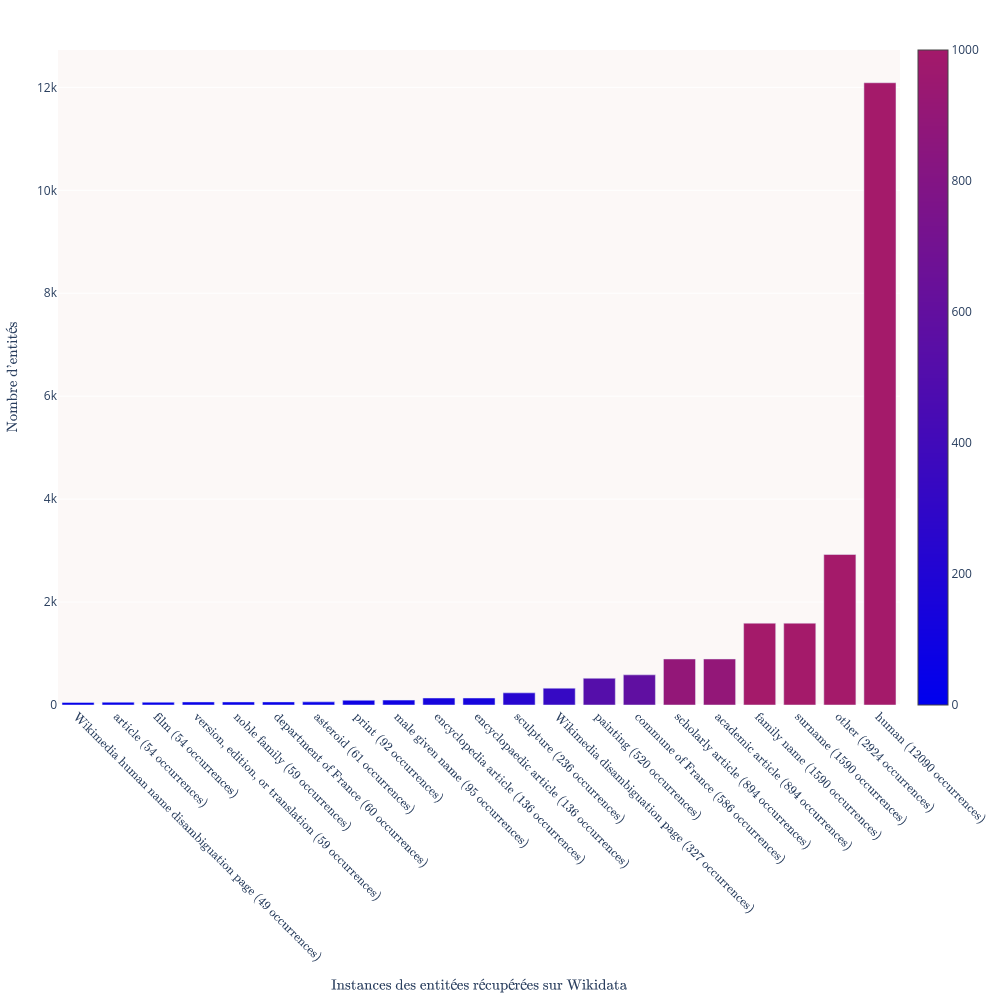
\includegraphics[width=\linewidth]{annexes/fig_wikidata_instances.png}
	\caption \\Occurrences des différentes catégories auxquelles appartiennent les entités \wkd{} liées avec les entrées de catalogues
	\label{appendix:wikidata_instances}
\end{figure}

\begin{figure}
	\centering
	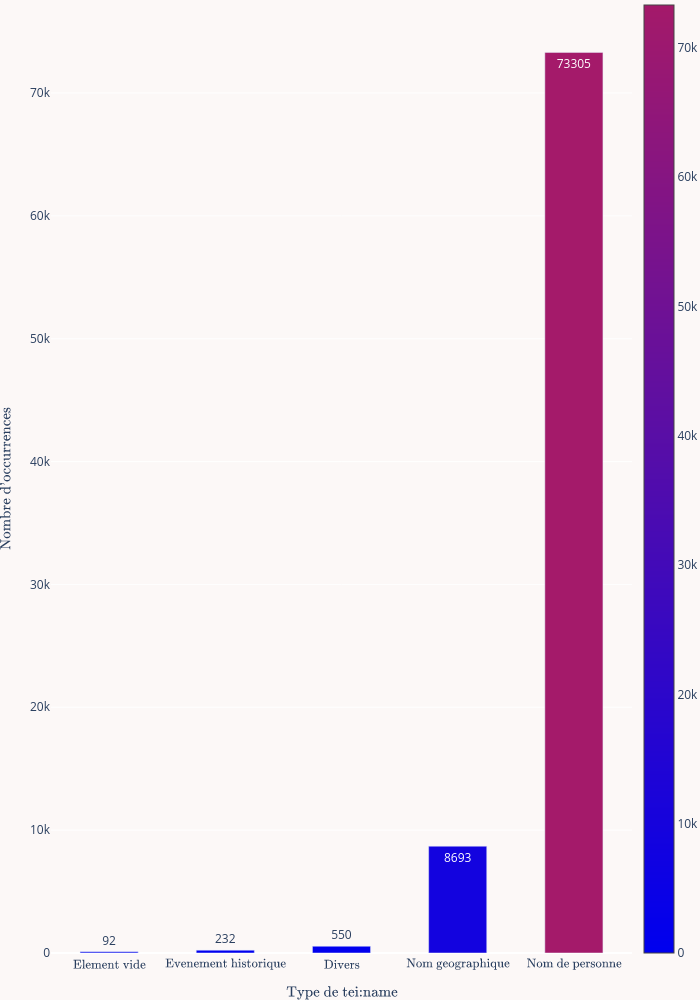
\includegraphics[width=\linewidth]{annexes/fig_teinametypes.png}
	\caption{Répartition des différents types de \tname{}}
	\label{appendix:tnametypes}
\end{figure}

\chapter{Code source et données encodées}
\begin{listing}
	\begin{minted}{python}
functions = {
	"général": "general",
	"maréchal": "marshal",
	"lieutenant": "military",
	"officier": "military",
	"colonel": "military",
	"lieutenant-colonel": "military",
	"commandant": "military",
	"capitaine": "military",  # "less important" military positions
	"roi": "king",
	"empereur": "emperor",
	"president": "president",
	"homme politique": "politician",
	"président de l'assemblée": "politician",
	"orateur": "politician",
	"député": "politician",
	"secrétaire d'état": "politician",
	"sénateur": "politician",
	"écrivain": "writer",
	"auteur": "writer",
	"romancier": "writer",
	"acteur": "actor",
	"actrice": "actress",
	"cantatrice": "singer",
	"chanteur": "singer",
	"chanteuse": "singer",
	"peintre": "painter",
	"sculpteur": "sculptor",
	"statutaire": "sculptor",
	"compositeur": "composer",
	"musicien": "musician",
	"musicienne": "musician",
	"tragédien": "actor",
	"chansonnier": "chansonnier",
	"achitecte": "architect",
	"journaliste": "journalist",
	"inventeur": "inventor",
	"chimiste": "chemist",
	"connétable": "constable",
	"archevêque": "archbishop",
	"évêque": "bishop",
	"docteur": "physicist",
	"médecin": "physicist"
}		
	\end{minted}
	\caption{Table de conversion associant un métier à son équivalent normalisé}
	\label{appendix:convfunction}
\end{listing}

	
\begin{listing}
	\begin{minted}{python}
dpts = [
	"ain",
	"aisne",
	"allier",
	"basses-alpes",
	"hautes-alpes",
	"alpes-maritimes",
	"annepins",
	"provence",
	"ardèche",
	"ardennes",
	"arriège",
	"arno",
	"aube",
	"aude",
	"aveyron",
	"bouches-de-l'elbe",
	"bouches-de-l'escaut",
	"bouches-de-l'yssel",
	"bpuches-de-la-meuse",
	"bouches-du-rhin",
	"bouches-du-rhône",
	"bouches-du-weser",
	"calvados",
	"cantal",
	"charente",
	"charente-inférieure",
	"cher",
	"corrèze",
	"corse",
	"côte-d'or",
	"côtes-du-nord",
	"creuse",
	"deux-nèthes",
	"deux-sèvres",
	"doire",
	"dordogne",
	"doubs",
	"drôme",
	"dyle",
	"ems-occidental",
	"ems-oriental",
	"ems-supérieur",
	"escaut",
	"eure",
	"eure-et-loir",
	"finistère",
	"forêts",
	"gard",
	"haute-garonne",
	"gers",
	"gironde",
	"hérault",
	"ille-et-villaine",
	"indre",
	"indre-et-loire",
	"isère",
	"jemappes",
	"jura",
	"landes",
	"léman",
	"loire",
	"loir-et-cher",
	"haute-loire",
	"loire-inférieure",
	"loiret",
	"lot",
	"lot-et-garonne",
	"lozère",
	"lys",
	"maine-et-loire",
	"manche",
	"marengo",
	"marne",
	"haute-marne",
	"méditerrannée",
	"mayenne",
	"meurthe",
	"meuse",
	"meuse-inférieure",
	"mont-blanc",
	"mont-tonnerre",
	"montenotte",
	"morbihan",
	"meuse",
	"moselle",
	"nièvre",
	"nord",
	"oise",
	"ombrone",
	"orne",
	"ourte",
	"paris",
	"pas-de-calais",
	"pô",
	"puy-de-dôme",
	"hautes-pyrénées",
	"basses-pyrénées",
	"pyrénées-orientales",
	"haut-rhin",
	"bas-rhin",
	"rhin-et-moselle",
	"rhône",
	"rhône-et-loire",
	"roer",
	"rome",
	"haute-saône",
	"saône-et-loire",
	"sambre-et-meuse",
	"sarre",
	"sarthe",
	"seine",
	"seine-et-marne",
	"seine-et-oise",
	"seine-inférieure",
	"sézia",
	"simplon",
	"deux-sèvres",
	"somme",
	"stura",
	"tarn",
	"tarn-et-garonne",
	"taro",
	"trasimène",
	"var",
	"vaucluse",
	"vendée",
	"vienne",
	"haute-vienne",
	"vosges",
	"yonne",
	"yssel-supérieur",
	"zuyderzée"
]		
	\end{minted}
	\caption{Liste de départements du XIXe~s. pour détecter des informations géographiques}
	\label{appendix:convdpt}
\end{listing}

\begin{listing}
	\begin{minted}{python}
countries = {
	"états-unis d'amérique": "united states of america",
	"etats-unis d'amérique": "united states of america",
	"états unis d'amérique": "united states of america",
	"etats unis d'amerique": "united states of america",
	"états-unis": "united states of america",
	"etats-unis": "united states of america",
	"etats unis": "united states of america",
	"états unis": "united states of america",
	"italie": "italy",
	"grèce": "greece",
	"canada": "canada",
	"chine": "china",
	"haïti": "haiti",
	"tobago": "tobago",
	"brésil": "brasil",
	"burkina-faso": "burkina-faso",
	"cameroun": "cameroun",
	"tchad": "tchad",
	"congo": "congo",
	"gabon": "gabon",
	"guinée": "guinea",
	"côte d'ivoire": "ivory coast",
	"mali": "mali",
	"mauritanie": "mauritania",
	"niger": "niger",
	"sénégal": "senegal",
	"madagascar": "madagascar",
	"seychelles": "seychelles",
	"tanzanie": "tanzania",
	"zanzibar": "zanzibar",
	"liban": "lebanon",
	"syrie": "syria",
	"inde": "india",
	"laos": "laos",
	"viet-nâm": "vietnam"
}	
	\end{minted}
	\caption{Table de conversion pour les pays}
	\label{appendix:convcountry}
\end{listing}

\begin{listing}
	\begin{minted}{python}
colonies = [
	"québec",
	"ontario",
	"saint-pierre-et-miquelon",
	"mississippi",
	"missouri",
	"louisiane",
	"anguilla",
	"antigua",
	"dominique",
	"saint-domingue",
	"guadeloupe",
	"monsterrat",
	"saint-martin",
	"saint-barthélémy",
	"sainte-lucy",
	"saint-vincent-et-les-grenadines",
	"saint-eustache",
	"saint-christophe",
	"martinique"
	"guyane française",
	"guyane",
	"maroc",  # unfortunately the morocco referred to in XIXth century france is a french protectorate
	"algérie",  # same
	"algérie française",  # same
	"tunisie",  # same
	"fezzan",
	"dahomey",
	"haute-volta",
	"oubangui-chari",
	"congo français",
	"moyen-congo",
	"guinée française",
	"soudan français",
	"gorée",
	"tigi",
	"djibouti",
	"cheikh saïd",
	"comores",
	"fort-dauphin",
	"îles maurice",
	"mayotte",
	"la réunion",
	"îles éparses",
	"île amsterdam",
	"île saint-paul",
	"archipel crozet",
	"îles kerguelen",
	"castellorizo",
	"grand-liban",
	"sandjak d'alexandrette",
	"indes françaises",
	"pondichéry",
	"karikal",
	"yanaon",
	"mahé",
	"chanderngor",
	"tonkin",
	"annam",
	"cochinchine",
	"guangzhou wan",
	"shanghai",
	"guangzhou",
	"tianjin",
	"hankou",
	"clipperton",
	"nouvelle-calédonie",
	"polynésie française",
	"vanuatu",
	"nouvelles-hébrides",
"wallis et futuna"
]
	\end{minted}
	\caption{Liste d'anciennes colonies françaises pour la détection de motifs}
	\label{appendix:convcolonie}
\end{listing}

\begin{listing}
	\begin{minted}{python}
provinces = [
	"armagnac",
	"île-de-france",
	"berry",
	"orléanais",
	"normandie",
	"languedoc",
	"lyonnais",
	"dauphiné",
	"champagne",
	"aunis",
	"saintonge",
	"poitou",
	"guyenne et gascogne",
	"bourgogne",
	"picardie",
	"anjou",
	"provence",
	"angoumois",
	"bourbonnais",
	"marche",
	"bretagne",
	"maine",
	"touraine",
	"limousin",
	"comté de foix",
	"auvergne",
	"béarn",
	"alsace",
	"artois",
	"roussillon",
	"flandre française et hainaut français",
	"franche-comté",
	"lorraine et trois-évêchés",
	"corse",
	"nivernais",
]
	\end{minted}
	\caption{Liste d'anciennes provinces françaises pour la détection de motifs}
	\label{appendix:convprov}
\end{listing}

\begin{listing}
\begin{minted}{python}
events = {
	"défense nationale": "government of national defense",
	"defense nationale": "government of national defense",
	"révolution française": "french revolution",
	"revolution francaise": "french revolution",
	"guerre de trente ans": "thirty years' war 1618 1648",
	"guerre de cent ans": "hundred years' war 1337 1453",
	"guerre de sept ans": "seven years war 1756 1763",
	"guerre": "war",
	"insurrection": "war",
	"siège de mayence": "siege of mainz",
	"siège": "siege",
	"commune": "commune",
	"défense": "battle",
	"révolution": "revolution"
}
\end{minted}
	\caption{Table de conversion pour les évènements historiques}
	\label{appendix:convevt}
\end{listing}

\begin{listing}
\begin{minted}{python}
\end{minted}
\label{}
\caption{Liste de colonies pour la détection de motifs}
\end{listing}

\begin{listing}
\begin{minted}{python}
\end{minted}
\label{}
\caption{Liste de colonies pour la détection de motifs}
\end{listing}
	
	
	
	
	
	
	
	
	
	
\end{document}